%=======================================================================
% Multi-Agent Research Orchestrator --- Complete Hinglish Master Notes (65+ Pages)
% ALL 10 Files Line-by-Line | RAG + MCP Deep Dive | 50 Interview Q\&A
%=======================================================================
\documentclass[12pt, a4paper]{article}

% -- Packages ----------------------------------------------------------
\usepackage[utf8]{inputenc}
\usepackage[T1]{fontenc}
\usepackage{lmodern}
\usepackage[margin=0.9in]{geometry}
\usepackage[table,xcdraw]{xcolor}
\usepackage{listings}
\usepackage{tcolorbox}
\usepackage{enumitem}
\usepackage{hyperref}
\usepackage{fancyhdr}
\usepackage{titlesec}
\usepackage{graphicx}
\usepackage{booktabs}
\usepackage{longtable}
\usepackage{amsmath}
\usepackage{amssymb}
\usepackage{tikz}
\usetikzlibrary{shapes.geometric, arrows.meta, positioning, calc, decorations.pathmorphing}
\usepackage{multicol}
\usepackage{fancyvrb}
\usepackage{mdframed}
\usepackage{fontawesome5}
\usepackage{tabularx}
\usepackage{float}
\usepackage{caption}
\usepackage{subcaption}
\usepackage{wrapfig}
\usepackage{parskip}

\tcbuselibrary{listings, skins, breakable}

% -- Colors ------------------------------------------------------------
\definecolor{bg}{HTML}{1a1a2e}
\definecolor{codebg}{HTML}{0d1117}
\definecolor{codeframe}{HTML}{30363d}
\definecolor{keyword}{HTML}{ff79c6}
\definecolor{string}{HTML}{f1fa8c}
\definecolor{comment}{HTML}{6272a4}
\definecolor{function}{HTML}{50fa7b}
\definecolor{accentpurple}{HTML}{bd93f9}
\definecolor{accentblue}{HTML}{8be9fd}
\definecolor{accentorange}{HTML}{ffb86c}
\definecolor{accentred}{HTML}{ff5555}
\definecolor{accentgreen}{HTML}{50fa7b}
\definecolor{notebg}{HTML}{fff8e1}
\definecolor{tipbg}{HTML}{e8f5e9}
\definecolor{warnbg}{HTML}{fff3e0}
\definecolor{importantbg}{HTML}{e3f2fd}
\definecolor{deepbg}{HTML}{f3e5f5}
\definecolor{storybg}{HTML}{fce4ec}

% -- Code Listing Style ------------------------------------------------
\lstdefinestyle{pythonstyle}{
    language=Python,
    basicstyle=\small\ttfamily\color{white},
    backgroundcolor=\color{codebg},
    keywordstyle=\color{keyword}\bfseries,
    stringstyle=\color{string},
    commentstyle=\color{comment}\itshape,
    numberstyle=\tiny\color{comment},
    numbers=left,
    numbersep=8pt,
    frame=single,
    rulecolor=\color{codeframe},
    breaklines=true,
    breakatwhitespace=false,
    showstringspaces=false,
    tabsize=4,
    captionpos=b,
    morekeywords={self, True, False, None, as, with, yield, async, await, f},
    emph={ResearchState, ChatGroq, TavilySearch, StateGraph, END, Chroma, FastMCP,
          HuggingFaceEmbeddings, PyPDFLoader, RecursiveCharacterTextSplitter,
          Document, TypedDict, Annotated},
    emphstyle=\color{accentblue}\bfseries,
    emph={[2]researcher_node, analyst_node, fact_checker_node, writer_node,
          build_graph, should_continue, get_embeddings, get_vectorstore,
          ingest_documents, retrieve_context, store_research_session,
          research_topic, ingest_document, search_knowledge_base},
    emphstyle={[2]\color{accentgreen}},
    literate={->}{{\textcolor{accentorange}{$\rightarrow$}}}1
             {<-}{{\textcolor{accentorange}{$\leftarrow$}}}1,
}

\lstdefinestyle{envstyle}{
    basicstyle=\small\ttfamily\color{white},
    backgroundcolor=\color{codebg},
    frame=single,
    rulecolor=\color{codeframe},
    breaklines=true,
    numbers=left,
    numberstyle=\tiny\color{comment},
    numbersep=8pt,
    commentstyle=\color{comment}\itshape,
    morecomment=[l]{\#},
}

\lstdefinestyle{bashstyle}{
    basicstyle=\small\ttfamily\color{accentgreen},
    backgroundcolor=\color{codebg},
    frame=single,
    rulecolor=\color{codeframe},
    breaklines=true,
    numbers=none,
}

\lstdefinestyle{cssstyle}{
    basicstyle=\small\ttfamily\color{white},
    backgroundcolor=\color{codebg},
    frame=single,
    rulecolor=\color{codeframe},
    breaklines=true,
    numbers=left,
    numberstyle=\tiny\color{comment},
    numbersep=8pt,
    keywordstyle=\color{accentblue}\bfseries,
    stringstyle=\color{string},
    commentstyle=\color{comment}\itshape,
    morecomment=[l]{//},
    morekeywords={background, color, border, padding, margin, font, display, flex, linear-gradient, rgba, transition, animation, transform, box-shadow},
}

% -- tcolorbox Styles --------------------------------------------------
\newtcolorbox{notebox}[1][]{
    colback=notebg, colframe=accentorange!70!black,
    fonttitle=\bfseries, title={\faIcon{lightbulb} ~Yaad Rakhne Ka Tip},
    rounded corners, breakable, #1
}
\newtcolorbox{conceptbox}[1][]{
    colback=importantbg, colframe=accentblue!70!black,
    fonttitle=\bfseries, title={\faIcon{brain} ~Concept Deep Dive},
    rounded corners, breakable, #1
}
\newtcolorbox{storybox}[1][]{
    colback=storybg, colframe=accentred!60!black,
    fonttitle=\bfseries, title={\faIcon{book-open} ~Kahani Se Samjho},
    rounded corners, breakable, #1
}
\newtcolorbox{warningbox}[1][]{
    colback=warnbg, colframe=accentorange!80!black,
    fonttitle=\bfseries, title={\faIcon{exclamation-triangle} ~Dhyan Do},
    rounded corners, breakable, #1
}
\newtcolorbox{interviewbox}[1][]{
    colback=deepbg, colframe=accentpurple!70!black,
    fonttitle=\bfseries, title={\faIcon{user-tie} ~Interview Question},
    rounded corners, breakable, #1
}
\newtcolorbox{codestorybox}[1][]{
    colback=tipbg, colframe=accentgreen!70!black,
    fonttitle=\bfseries, title={\faIcon{code} ~Code Samjho Line-by-Line},
    rounded corners, breakable, #1
}
\newtcolorbox{mathbox}[1][]{
    colback=importantbg, colframe=accentblue!60!black,
    fonttitle=\bfseries, title={\faIcon{square-root-alt} ~Maths Behind the Scene},
    rounded corners, breakable, #1
}
\newtcolorbox{memorybox}[1][]{
    colback=notebg, colframe=accentorange!60!black,
    fonttitle=\bfseries, title={\faIcon{memory} ~Memory Trick},
    rounded corners, breakable, #1
}

% -- Page Style --------------------------------------------------------
\pagestyle{fancy}
\fancyhf{}
\fancyhead[L]{\textcolor{accentpurple}{\small\textbf{Multi-Agent Research Orchestrator}}}
\fancyhead[R]{\textcolor{comment}{\small Master Hinglish Notes}}
\fancyfoot[C]{\textcolor{accentblue}{\thepage}}
\renewcommand{\headrulewidth}{0.4pt}
\renewcommand{\headrule}{\hbox to\headwidth{\color{accentpurple}\leaders\hrule height \headrulewidth\hfill}}

% -- Section Formatting ------------------------------------------------
\titleformat{\section}{\LARGE\bfseries\color{accentpurple}}{
    \colorbox{accentpurple!15}{\makebox[2em]{\thesection}}}{0.5em}{}[
    \vspace{-0.5em}\color{accentpurple}\rule{\textwidth}{2pt}]

\titleformat{\subsection}{\Large\bfseries\color{accentblue}}{
    \thesubsection}{0.5em}{}[\vspace{-0.3em}\color{accentblue!40}\rule{0.7\textwidth}{0.5pt}]

\titleformat{\subsubsection}{\large\bfseries\color{accentorange}}{
    \thesubsubsection}{0.5em}{}

% -- Hyperref Setup ----------------------------------------------------
\hypersetup{
    colorlinks=true,
    linkcolor=accentpurple,
    urlcolor=accentblue,
    citecolor=accentgreen,
    bookmarks=true,
    bookmarksopen=true,
}

% -- Document Start ----------------------------------------------------
\begin{document}

% ======================================================================
% TITLE PAGE
% ======================================================================
\begin{titlepage}
\begin{center}
\vspace*{1cm}

\begin{tikzpicture}
  \node[circle, draw=accentpurple, line width=3pt, minimum size=3cm,
        fill=accentpurple!10] (center) {
    \Huge\color{accentpurple}\faIcon{microscope}
  };
  \foreach \angle/\icon/\col in {
    45/\faIcon{search}/accentblue,
    135/\faIcon{chart-bar}/accentgreen,
    225/\faIcon{check-circle}/accentorange,
    315/\faIcon{pen-fancy}/accentred%
  }{
    \node[circle, draw=\col, line width=2pt, minimum size=1.8cm,
          fill=\col!10] at (\angle:3.5cm) {\Large\color{\col}\icon};
    \draw[-{Stealth[length=3mm]}, \col, line width=1.5pt]
          (center.\angle) -- (\angle:2.5cm);
  }
\end{tikzpicture}

\vspace{1.5cm}
{\Huge\bfseries\color{accentpurple} Multi-Agent Research Orchestrator}\\[0.5cm]
{\LARGE\color{accentblue} Complete Hinglish Master Notes}\\[0.3cm]
{\large\color{comment} 65+ Pages $\bullet$ Line-by-Line Code Explanation $\bullet$ 50 Interview Q\&A}\\[0.3cm]
{\large\color{comment} RAG $\bullet$ MCP $\bullet$ LangGraph $\bullet$ Groq $\bullet$ ChromaDB $\bullet$ Streamlit}

\vspace{1.5cm}

\begin{tikzpicture}
\node[draw=accentblue!50, rounded corners=10pt, fill=accentblue!5,
      text width=14cm, align=center, inner sep=15pt] {
    \color{accentblue}\large\textbf{Tech Stack at a Glance}\\[8pt]
    \begin{tabular}{ll}
    \color{keyword}\faIcon{brain} \textbf{LLM} & Groq (GPT-OSS-120B) \\
    \color{accentgreen}\faIcon{project-diagram} \textbf{Orchestration} & LangGraph StateGraph \\
    \color{accentorange}\faIcon{search} \textbf{Web Search} & Tavily (Advanced Depth) \\
    \color{accentblue}\faIcon{database} \textbf{Vector Store} & ChromaDB (Persistent) \\
    \color{string}\faIcon{robot} \textbf{Embeddings} & HuggingFace all-MiniLM-L6-v2 (Free, Local) \\
    \color{accentred}\faIcon{desktop} \textbf{UI} & Streamlit (Glassmorphism Dark Theme) \\
    \color{accentpurple}\faIcon{plug} \textbf{Protocol} & MCP (Model Context Protocol) via FastMCP \\
    \color{function}\faIcon{python} \textbf{Language} & Python 3.10+ \\
    \end{tabular}
};
\end{tikzpicture}

\vfill
{\color{comment}\today}
\end{center}
\end{titlepage}

% ======================================================================
% TABLE OF CONTENTS
% ======================================================================
\tableofcontents
\newpage

% ######################################################################
%  SECTION 1: PROJECT OVERVIEW - KAHANI KI SHURUAAT
% ######################################################################
\section{Project Overview --- Kahani Ki Shuruaat}

\begin{storybox}
Socho tumhe ek aisa system banana hai jo kisi bhi topic par research kar sake --- jaise ek team of 4 experts kaam karti hai:

\begin{enumerate}[label=\textcolor{accentpurple}{\arabic*.}]
\item \textbf{Researcher (Khoji):} Internet par search karta hai, data collect karta hai. Jaise ek journalist jo field mein jata hai.
\item \textbf{Analyst (Vishleshan-karta):} Collected data ko analyze karta hai --- patterns dhundhta hai, contradictions nikalta hai. Jaise ek detective jo clues jodta hai.
\item \textbf{Fact Checker (Satya-parikshak):} Claims verify karta hai --- kya sab sach hai? Agar kuch galat hai, toh wapas Researcher ko bhejta hai. Jaise ek editor jo facts check karta hai.
\item \textbf{Writer (Lekhak):} Sab verified data ko ek polished report mein likhta hai with citations. Jaise ek professional writer.
\end{enumerate}

Ab ye 4 agents ek pipeline mein kaam karte hain: \\
\textbf{Researcher $\rightarrow$ Analyst $\rightarrow$ Fact-Checker $\rightarrow$ Writer} \\
Aur ek \textbf{feedback loop} hai --- agar Fact-Checker ko kuch galat milta hai, toh wapas Researcher ko bhejta hai (max 2 baar). \\[6pt]
Is project mein humne \textbf{RAG (Retrieval Augmented Generation)} bhi add kiya hai --- matlab tum apne PDF documents upload kar sakte ho aur agents unhe bhi search karenge. Plus \textbf{MCP (Model Context Protocol)} se ye system kisi bhi AI tool (Claude Desktop, Cursor) se connect ho sakta hai!
\end{storybox}

\subsection{Project Architecture Diagram}

\begin{center}
\begin{tikzpicture}[
    node distance=2.5cm and 3cm,
    box/.style={draw=#1, rounded corners=8pt, fill=#1!10, text width=3.5cm,
                align=center, minimum height=1.5cm, font=\small\bfseries,
                line width=1.5pt},
    arrow/.style={-{Stealth[length=4mm]}, line width=2pt, #1},
    label/.style={font=\tiny\color{comment}, align=center}
]
    % Nodes
    \node[box=accentpurple] (user) {USER\\{\small\color{comment}Topic Input}};
    \node[box=accentblue, right=of user] (res) {RESEARCHER\\{\small\color{comment}Tavily + RAG}};
    \node[box=accentgreen, right=of res] (ana) {ANALYST\\{\small\color{comment}Themes + Gaps}};
    \node[box=accentorange, below=2cm of ana] (fc) {FACT CHECKER\\{\small\color{comment}Verify Claims}};
    \node[box=accentred, left=of fc] (wr) {WRITER\\{\small\color{comment}Report + Citations}};
    \node[box=accentpurple!70, left=of wr] (out) {OUTPUT\\{\small\color{comment}Markdown Report}};

    % Edges
    \draw[arrow=accentpurple] (user) -- (res) node[midway,above,label] {topic};
    \draw[arrow=accentblue] (res) -- (ana) node[midway,above,label] {research\_data};
    \draw[arrow=accentgreen] (ana) -- (fc) node[midway,right,label] {analysis};
    \draw[arrow=accentorange] (fc) -- (wr) node[midway,above,label] {PASSED};
    \draw[arrow=accentred] (wr) -- (out) node[midway,above,label] {final\_report};

    % Feedback loop
    \draw[arrow=accentred!70, dashed, line width=1.5pt]
        (fc.west) -- ++(-1,0) |- node[near start, left, label] {NEEDS\\REVISION}
        (res.south);

    % RAG + ChromaDB
    \node[draw=accentorange, dashed, rounded corners=5pt, fill=accentorange!5,
          below=1.2cm of res, text width=2.8cm, align=center, font=\small]
          (chroma) {ChromaDB\\{\tiny Vector Store}};
    \draw[{Stealth[length=2mm]}-{Stealth[length=2mm]}, accentorange, dashed]
        (res.south) -- (chroma.north) node[midway,right,label] {RAG};
\end{tikzpicture}
\end{center}

\subsection{Folder Structure}

Project ka folder structure samajhna bahut zaroori hai. Ye ek clean, modular structure hai:

\begin{lstlisting}[style=bashstyle]
Multi-Agent-Research-Orchestrator/
|-- app.py                  # Streamlit UI (707 lines)
|-- mcp_server.py           # MCP Protocol Server (208 lines)
|-- requirements.txt        # Dependencies
|-- .env.example            # API keys template
|-- .gitignore
|--
|-- config/
|   |-- __init__.py
|   |-- setting.py         # Centralized configuration (42 lines)
|--
|-- state/
|   |-- __init__.py
|   |-- schema.py           # Shared state TypedDict (59 lines)
|--
|-- agents/
|   |-- __init__.py
|   |-- researcher.py       # Web Search + RAG Agent (121 lines)
|   |-- analyst.py          # Analysis Agent (85 lines)
|   |-- fact_checker.py     # Verification Agent (107 lines)
|   |-- writer.py           # Report Writer Agent (135 lines)
|--
|-- graph/
|   |-- __init__.py
|   |-- workflow.py          # LangGraph Pipeline (78 lines)
|--
|-- rag/
|   |-- __init__.py
|   |-- vector_store.py      # ChromaDB RAG Manager (276 lines)
\end{lstlisting}

\begin{notebox}
\textbf{Yaad Rakho:} Har folder mein \texttt{\_\_init\_\_.py} file hoti hai --- ye Python ko batati hai ki ``ye ek package hai, isko import kar sakte ho.'' Bina iske \texttt{from agents.researcher import ...} kaam nahi karega!
\end{notebox}

\subsection{Dependencies Explained (requirements.txt)}

Pehle samjho hum kya install kar rahe hain aur \textbf{kyun}:

\begin{lstlisting}[style=pythonstyle, title={\color{accentgreen}\faIcon{file} requirements.txt}]
# Core LangChain Framework
langchain>=0.3.0              # Base framework for LLM apps
langchain-groq>=0.3.0         # Groq LLM integration
langchain-tavily>=0.1.0       # Tavily search tool wrapper
langchain-community>=0.3.0    # Community integrations
langgraph>=0.4.0              # StateGraph for multi-agent
streamlit>=1.40.0             # Web UI framework
python-dotenv>=1.0.0          # .env file loader
pydantic>=2.0.0               # Data validation

# RAG Dependencies
langchain-chroma>=0.2.0       # ChromaDB vector store
langchain-huggingface>=0.1.0  # HuggingFace embeddings
langchain-text-splitters>=0.3.0  # Text chunking
pypdf>=5.0.0                  # PDF file reader

# MCP Dependencies
fastmcp>=2.0.0                # MCP protocol server
\end{lstlisting}

\begin{codestorybox}
\textbf{Har dependency ka role:}
\begin{itemize}[leftmargin=*]
\item \texttt{langchain} --- Ye ``spine'' hai puri app ki. LLM calls, prompts, chains --- sab iske through.
\item \texttt{langchain-groq} --- Groq ka LLM use karne ke liye. Groq ultra-fast hai (custom hardware pe LLaMA run karta hai).
\item \texttt{langchain-tavily} --- Tavily ek AI-optimized search engine hai. Google API se zyada structured data deta hai.
\item \texttt{langgraph} --- Multi-agent workflow banane ke liye. Ye ``graph'' based hai --- nodes (agents) aur edges (connections).
\item \texttt{streamlit} --- Python se web app banane ka sabse easy tarika. No HTML/JS needed (mostly).
\item \texttt{langchain-chroma} --- ChromaDB vector database. Documents ko vectors mein store karta hai for semantic search.
\item \texttt{langchain-huggingface} --- HuggingFace se embedding models load karne ke liye. Free aur local.
\item \texttt{pypdf} --- PDF files ko text mein convert karne ke liye.
\item \texttt{fastmcp} --- MCP protocol server banane ke liye. Claude Desktop, Cursor jaisi tools se connect.
\end{itemize}
\end{codestorybox}


% ######################################################################
%  SECTION 2: CONFIGURATION - SETTINGS.PY
% ######################################################################
\newpage
\section{Configuration --- \texttt{config/setting.py}}

\begin{storybox}
Socho tumhare ghar mein ek \textbf{control panel} hai --- AC ka temperature, lights ka brightness, wifi ka password --- sab ek jagah se control hota hai. \texttt{setting.py} exactly wahi hai --- \textbf{saari configuration ek jagah}, taki agar kuch change karna ho toh sirf ek file mein karo. Isko kehte hain \textbf{``Single Source of Truth''}.
\end{storybox}

\subsection{Complete Code with Line-by-Line Explanation}

\begin{lstlisting}[style=pythonstyle, title={\color{accentgreen}\faIcon{file} config/setting.py --- Full Code}]
"""
Centralized configuration -- loads .env and exposes settings.
"""

import os                        # Line 5
from dotenv import load_dotenv   # Line 6

# Load environment variables from .env file
load_dotenv()                    # Line 9


def get_env_var(key: str, default: str | None = None,
                required: bool = False) -> str:
    """Get an environment variable with optional default
       and requirement check."""
    value = os.getenv(key, default)        # Line 15
    if required and not value:             # Line 16
        raise ValueError(                  # Line 17
            f"Missing required environment variable: {key}\n"
            f"Please set it in your .env file. "
            f"See .env.example for reference."
        )
    return value or ""                     # Line 21


# -- API Keys -----------------------------------------
GROQ_API_KEY = get_env_var("GROQ_API_KEY", required=True)
TAVILY_API_KEY = get_env_var("TAVILY_API_KEY", required=True)

# -- Model Configuration ------------------------------
MODEL_NAME = get_env_var("MODEL_NAME",
                         default="openai/gpt-oss-120b")
MAX_SEARCH_RESULTS = int(get_env_var("MAX_SEARCH_RESULTS",
                                      default="5"))
MAX_REVISIONS = int(get_env_var("MAX_REVISIONS", default="2"))

# -- RAG Configuration ---------------------------------
CHROMA_PERSIST_DIR = get_env_var("CHROMA_PERSIST_DIR",
                                  default="./chroma_db")
EMBEDDING_MODEL = get_env_var("EMBEDDING_MODEL",
    default="sentence-transformers/all-MiniLM-L6-v2")
CHUNK_SIZE = int(get_env_var("CHUNK_SIZE", default="1000"))
CHUNK_OVERLAP = int(get_env_var("CHUNK_OVERLAP", default="200"))

# -- Set keys in environment (required by LangChain) ---
os.environ["GROQ_API_KEY"] = GROQ_API_KEY
os.environ["TAVILY_API_KEY"] = TAVILY_API_KEY
\end{lstlisting}

\begin{codestorybox}
\textbf{Line-by-Line Breakdown:}

\textbf{Line 5: \texttt{import os}} --- Python ka built-in module. System se baat karne ke liye --- files read karo, environment variables lo, paths banao.

\textbf{Line 6: \texttt{from dotenv import load\_dotenv}} --- \texttt{python-dotenv} library se aata hai. Ye \texttt{.env} file ko padhkar environment variables set karta hai. Matlab tumhara API key code mein hardcode nahi hoga (security best practice!).

\textbf{Line 9: \texttt{load\_dotenv()}} --- Ye function call karte hi, ye \texttt{.env} file dhundhta hai project root mein, usko padhta hai, aur har line ko \texttt{os.environ} mein daal deta hai. Example:
\begin{verbatim}
  .env file mein:  GROQ_API_KEY=gsk_abc123xyz
  Ab Python mein:  os.getenv("GROQ_API_KEY") => "gsk_abc123xyz"
\end{verbatim}

\textbf{Lines 12-21: \texttt{get\_env\_var()} function} --- Ye ek helper function hai jo environment variable padhta hai with error handling:
\begin{itemize}[leftmargin=*]
\item \texttt{key: str} --- Variable ka naam, e.g., ``GROQ\_API\_KEY''
\item \texttt{default: str | None = None} --- Agar variable nahi mila toh ye value use karo
\item \texttt{required: bool = False} --- Agar \texttt{True} hai aur variable nahi mila, toh \texttt{ValueError} raise karo (app crash with clear message)
\item \texttt{str | None} --- Ye Python 3.10+ ka ``union type'' hai. Pehle \texttt{Optional[str]} likhte the.
\end{itemize}

\textbf{Line 24-25: API Keys} --- Ye \textbf{required=True} hain. Matlab agar \texttt{.env} mein ye keys nahi hain, toh app start hi nahi hogi. Ye deliberate hai --- bina API keys ke agents kuch kar hi nahi sakte.

\textbf{Lines 28-31: Model Config} --- \texttt{MODEL\_NAME} default ``openai/gpt-oss-120b'' hai. Isko \texttt{.env} se override kar sakte ho. \texttt{MAX\_SEARCH\_RESULTS} aur \texttt{MAX\_REVISIONS} ko \texttt{int()} mein wrap kiya kyunki env vars hamesha string hote hain.

\textbf{Lines 33-37: RAG Config} --- ChromaDB kahan save hoga, kaunsa embedding model use hoga, chunks kitne bade honge --- ye sab configurable hai.

\textbf{Lines 39-40: Set in os.environ} --- LangChain integrations apne se \texttt{os.environ} se keys read karti hain. Toh hum explicitly set karte hain taaki koi issue na aaye.
\end{codestorybox}

\begin{notebox}
\textbf{Syntax Yaad Karo:}
\begin{lstlisting}[style=pythonstyle]
# Environment variable padhne ka pattern:
import os
from dotenv import load_dotenv
load_dotenv()
api_key = os.getenv("MY_KEY", "default_value")

# Type hint with union (Python 3.10+):
def func(x: str | None = None) -> str:
    return x or "fallback"
\end{lstlisting}
\end{notebox}

\begin{conceptbox}[title={\faIcon{brain} ~Why \texttt{.env} Files?}]
\textbf{Security:} API keys ko code mein likhna bohot bura practice hai. Agar tum code ko GitHub pe push karte ho, toh koi bhi tumhare keys chura sakta hai. \texttt{.env} file ko \texttt{.gitignore} mein daalo taki ye kabhi Git repo mein na jaaye.

\textbf{Flexibility:} Development aur production mein different keys chahiye? Bas alag \texttt{.env} files use karo. Code change ki zaroorat nahi.

\textbf{Team Work:} \texttt{.env.example} file share karo (bina actual keys ke). Naye developer ko pata chal jayega ki kaunsi keys chahiye.
\end{conceptbox}


% ######################################################################
%  SECTION 3: STATE SCHEMA
% ######################################################################
\newpage
\section{State Schema --- \texttt{state/schema.py}}

\begin{storybox}
Socho 4 doctors ek patient ka ilaaj kar rahe hain. Unhe ek \textbf{shared medical file} chahiye jismein saari information ho --- symptoms, test results, diagnosis, treatment plan. Agar har doctor apni alag file rakhega, toh confusion hoga.

\texttt{ResearchState} exactly wahi \textbf{shared file} hai --- ye ek TypedDict hai jo define karta hai ki pipeline mein kya-kya data flow karega. Har agent isko padh sakta hai aur update kar sakta hai.
\end{storybox}

\subsection{Complete Code with Explanation}

\begin{lstlisting}[style=pythonstyle, title={\color{accentgreen}\faIcon{file} state/schema.py --- Full Code}]
"""
Shared state schema for the multi-agent research pipeline.

Uses TypedDict with Annotated reducer fields so that multiple
agents can safely append to list fields without overwriting
each other.
"""

from __future__ import annotations     # Line 8
import operator                         # Line 10
from typing import Annotated, TypedDict # Line 11


class ResearchState(TypedDict):
    """Central state shared across all agents."""

    # -- User Input ----
    topic: str
    """The user's research query / topic."""

    # -- Researcher Output ----
    research_data: Annotated[list[str], operator.add]
    """Raw search results collected by the Researcher agent.
    Uses operator.add reducer -- each agent call *appends*."""

    # -- Analyst Output ----
    analysis: str
    """Structured analysis with key themes, patterns."""

    # -- Fact-Checker Output ----
    fact_check_result: str
    """Detailed fact-check report."""

    fact_check_passed: bool
    """Gate flag -- True = proceed, False = loop back."""

    revision_count: int
    """Number of research->fact-check loops. Capped."""

    # -- Writer Output ----
    final_report: str
    """The polished, cited markdown report."""

    # -- RAG Context ----
    rag_context: Annotated[list[str], operator.add]
    """Context from uploaded documents via ChromaDB RAG."""

    # -- Pipeline Metadata ----
    messages: Annotated[list[str], operator.add]
    """Running log of agent activity messages."""

    current_agent: str
    """Name of the currently active agent."""

    error: str
    """Error message if something goes wrong."""
\end{lstlisting}

\begin{codestorybox}
\textbf{Line-by-Line Deep Dive:}

\textbf{Line 8: \texttt{from \_\_future\_\_ import annotations}} --- Ye ek ``magic import'' hai. Isse Python type hints ko ``lazy'' banata hai --- matlab type hints runtime pe evaluate nahi hote, sirf static analysis ke liye hote hain. Iska fayda: tum \texttt{list[str]} jaise modern syntax use kar sakte ho Python 3.9 mein bhi.

\textbf{Line 10: \texttt{import operator}} --- Python ka built-in module for operators as functions. \texttt{operator.add} matlab \texttt{+} operator as a function. Ye LangGraph ko batata hai ``list fields ko merge (concatenate) karo, overwrite mat karo.''

\textbf{Line 11: \texttt{from typing import Annotated, TypedDict}} ---
\begin{itemize}[leftmargin=*]
\item \texttt{TypedDict}: Ye ek special dict hai jismein har key ka type defined hota hai. Normal dict mein kuch bhi daal sakte ho, but TypedDict mein sirf defined keys allowed hain.
\item \texttt{Annotated}: Ye type hints mein extra metadata attach karne ka mechanism hai. Yahan hum ``reducer function'' attach kar rahe hain.
\end{itemize}

\textbf{Line 14: \texttt{class ResearchState(TypedDict):}} --- Ye humara \textbf{state container} hai. LangGraph mein har node (agent) ko ye state milti hai as input aur ye state return karti hai as output.
\end{codestorybox}

\begin{conceptbox}[title={\faIcon{brain} ~Annotated Reducer --- Core LangGraph Concept}]
Ye sabse important concept hai is project mein. Samjho carefully:

\textbf{Problem:} Agar Researcher agent \texttt{messages = ["msg1"]} return kare, aur Analyst agent \texttt{messages = ["msg2"]} return kare --- toh kya hoga? Normal dict mein ``msg1'' overwrite ho jayega!

\textbf{Solution: Reducer Pattern}
\begin{lstlisting}[style=pythonstyle]
# BIN Reducer (default behavior):
messages = ["msg2"]  # Analyst ne Researcher ka data uda diya!

# WITH Reducer (operator.add):
messages: Annotated[list[str], operator.add]
# Ab: messages = ["msg1"] + ["msg2"] = ["msg1", "msg2"]
# Dono preserve hote hain!
\end{lstlisting}

\textbf{Kaise kaam karta hai internally?}

Jab LangGraph ek node ka output process karta hai:
\begin{enumerate}
\item Check karta hai --- kya is field pe \texttt{Annotated} with reducer hai?
\item Agar haan --- toh \texttt{reducer(old\_value, new\_value)} call karta hai
\item \texttt{operator.add} for lists: \texttt{[old] + [new]} = concatenation
\item Agar nahi --- toh simply overwrite karta hai (last write wins)
\end{enumerate}
\end{conceptbox}

\begin{mathbox}
\textbf{State Evolution Formula:}

Maan lo $S_t$ state hai time $t$ pe, aur agent $A_i$ output deta hai $\Delta_i$:

\begin{align}
S_{t+1}[\text{topic}] &= \Delta_i[\text{topic}] \quad \text{(overwrite --- no reducer)} \\
S_{t+1}[\text{messages}] &= S_t[\text{messages}] \oplus \Delta_i[\text{messages}] \quad \text{(append --- operator.add)} \\
\text{where } \oplus &\equiv \text{list concatenation (operator.add)}
\end{align}

Matlab \texttt{topic} hamesha latest value rakhega (overwrite), lekin \texttt{messages} sab accumulate hote rahenge (append).
\end{mathbox}

\begin{memorybox}
\textbf{Yaad Rakhne Ka Trick:} \\
``\textbf{A}nnotated = \textbf{A}ppend, Normal = \textbf{N}ew (overwrite)'' \\[4pt]
Jab bhi list field mein sabka data rakhna ho $\rightarrow$ \texttt{Annotated[list, operator.add]} \\
Jab sirf latest value chahiye $\rightarrow$ normal type hint (\texttt{str}, \texttt{bool}, etc.)
\end{memorybox}

\subsection{State Fields Ka Role Table}

\begin{center}
\small
\begin{longtable}{|>{\ttfamily\small}p{3.5cm}|p{2cm}|p{2cm}|p{5.5cm}|}
\hline
\rowcolor{accentpurple!15}
\textbf{Field} & \textbf{Type} & \textbf{Reducer?} & \textbf{Purpose (Hinglish)} \\
\hline\hline
topic & str & No & User ne kya research karna hai \\
\hline
research\_data & list[str] & operator.add & Web search ke results, har baar append \\
\hline
analysis & str & No & Analyst ka structured output \\
\hline
fact\_check\_result & str & No & Fact checker ka detailed report \\
\hline
fact\_check\_passed & bool & No & True = Writer pe jao, False = wapas Researcher \\
\hline
revision\_count & int & No & Kitni baar loop hua (max 2) \\
\hline
final\_report & str & No & Writer ka final markdown report \\
\hline
rag\_context & list[str] & operator.add & ChromaDB se mile document chunks \\
\hline
messages & list[str] & operator.add & UI ke liye activity log \\
\hline
current\_agent & str & No & Abhi kaunsa agent active hai \\
\hline
error & str & No & Koi error aaya toh yahan store \\
\hline
\end{longtable}
\end{center}


% ######################################################################
%  SECTION 4: RESEARCHER AGENT
% ######################################################################
\newpage
\section{Researcher Agent --- \texttt{agents/researcher.py}}

\begin{storybox}
Researcher agent ek \textbf{investigative journalist} jaisa hai. Usko topic milta hai, woh:
\begin{enumerate}
\item Pehle \textbf{3 strategic sub-queries} generate karta hai (LLM se)
\item Phir har query ke liye \textbf{Tavily web search} karta hai
\item Saath mein \textbf{ChromaDB mein uploaded documents} bhi search karta hai (RAG)
\item Aur \textbf{past research memory} bhi check karta hai
\item Sab results ko aggregate karke return karta hai
\end{enumerate}
Agar ye revision round hai (Fact Checker ne wapas bheja), toh queries fact-checker feedback pe based hoti hain.
\end{storybox}

\subsection{Complete Code with Detailed Commentary}

\begin{lstlisting}[style=pythonstyle, title={\color{accentgreen}\faIcon{file} agents/researcher.py --- Full Code (121 lines)}]
"""
Researcher Agent
-----------------
Uses Tavily web search AND ChromaDB RAG to gather data.
Strategy: generates 3 strategic sub-queries from the main
topic, then searches BOTH web and uploaded documents.
"""

from langchain_groq import ChatGroq              # Line 10
from langchain_tavily import TavilySearch         # Line 11
from langchain_core.messages import (             # Line 12
    SystemMessage, HumanMessage
)

from config.settings import MODEL_NAME, MAX_SEARCH_RESULTS
from state.schema import ResearchState            # Line 16


# -- Tool setup ----------------------------------------
search_tool = TavilySearch(                       # Line 19
    max_results=MAX_SEARCH_RESULTS,               # Line 20
    search_depth="advanced",                      # Line 21
)

llm = ChatGroq(model=MODEL_NAME, temperature=0)   # Line 24


def researcher_node(state: ResearchState) -> dict: # Line 27
    """
    Researcher agent node for the LangGraph pipeline.
    """
    topic = state["topic"]                         # Line 31
    revision_count = state.get("revision_count", 0) # Line 32

    # If revision loop, use fact-checker feedback
    if revision_count > 0 and state.get("fact_check_result"):
        query_prompt = f"""You are a research strategist.
A fact-checker has flagged issues with previous research
on: "{topic}"

Fact-checker feedback:
{state['fact_check_result']}

Generate exactly 3 targeted search queries to fill the
gaps and verify the flagged claims. Return ONLY the 3
queries, one per line, no numbering or bullets."""
    else:
        query_prompt = f"""You are a research strategist.
Generate exactly 3 focused, diverse search queries to
comprehensively research this topic: "{topic}"

Cover different angles: factual data, expert opinions,
and recent developments.
Return ONLY the 3 queries, one per line."""

    # Generate sub-queries via LLM
    query_response = llm.invoke([                  # Line 58
        SystemMessage(content="You are a research query "
                      "generator. Output only the queries."),
        HumanMessage(content=query_prompt),
    ])

    sub_queries = [q.strip() for q in              # Line 63
        query_response.content.strip().split("\n")
        if q.strip()]
    sub_queries = sub_queries[:3]  # Safety cap     # Line 65

    # Fallback if LLM fails
    if not sub_queries:                             # Line 68
        sub_queries = [topic]

    # -- Web Search (Tavily) ---------------------------
    all_results = []
    for query in sub_queries:                       # Line 72
        try:
            results = search_tool.invoke(           # Line 74
                {"query": query}
            )
            if isinstance(results, list):           # Line 76
                for r in results:
                    if isinstance(r, dict):
                        source = r.get("url",
                                       "Unknown source")
                        content = r.get("content", "")
                        all_results.append(
                            f"[Source: {source}]\n{content}"
                        )
                    else:
                        all_results.append(str(r))
            elif isinstance(results, str):
                all_results.append(results)
        except Exception as e:
            all_results.append(
                f"[Search error for '{query}']: {str(e)}"
            )

    # -- RAG Retrieval (ChromaDB) ----------------------
    rag_results = []
    try:
        from rag.vector_store import retrieve_context

        # Search uploaded documents
        doc_context = retrieve_context(             # Line 94
            topic,
            collection_name="research_docs",
            k=5
        )
        if doc_context:
            rag_results.extend(doc_context)

        # Search past research memory
        past_context = retrieve_context(            # Line 99
            topic,
            collection_name="past_research",
            k=3
        )
        if past_context:
            rag_results.extend(past_context)

    except Exception as e:
        rag_results.append(
            f"[RAG retrieval note]: {str(e)}"
        )

    # -- Status Message --------------------------------
    rag_count = len([r for r in rag_results
        if not r.startswith("[RAG retrieval note]")])
    status = (
        f"Researcher: Searched {len(sub_queries)} "
        f"web queries, found {len(all_results)} results"
        + (f" + {rag_count} RAG chunks"
           if rag_count > 0 else "")
        + (" (revision round)"
           if revision_count > 0 else "")
    )

    return {                                        # Line 115
        "research_data": all_results,
        "rag_context": rag_results,
        "messages": [status],
        "current_agent": "researcher",
    }
\end{lstlisting}

\begin{codestorybox}
\textbf{Critical Lines Explained:}

\textbf{Line 19-22: TavilySearch Setup}
\begin{itemize}[leftmargin=*]
\item \texttt{max\_results=MAX\_SEARCH\_RESULTS} --- Har query ke liye kitne results chahiye (default 5)
\item \texttt{search\_depth="advanced"} --- Tavily ka advanced mode. Ye zyada thorough search karta hai --- pages ke andar bhi content extract karta hai, sirf snippets nahi deta. Basic mode sirf surface-level results deta hai.
\end{itemize}

\textbf{Line 24: LLM Setup} --- \texttt{temperature=0} matlab \textbf{deterministic output}. Researcher ko creative nahi hona hai --- usko same input pe same queries generate karni hain. Temperature 0 se 1 tak hota hai:
\begin{itemize}
\item 0 = Same output every time (best for factual tasks)
\item 0.3 = Thoda variation (Writer agent mein use hota hai)
\item 1.0 = Maximum creativity (poetry, stories ke liye)
\end{itemize}

\textbf{Lines 34-55: Query Generation Strategy} --- Ye sabse clever part hai. Instead of directly searching the topic, hum LLM se 3 diverse sub-queries generate karte hain. Kyun?
\begin{itemize}
\item Ek hi query se limited perspective milti hai
\item 3 queries se ``factual data'', ``expert opinions'', ``recent developments'' --- teen alag angles cover hote hain
\item Revision round mein: Fact Checker ka feedback use karke \textbf{specific gaps} fill karte hain
\end{itemize}

\textbf{Line 63-65: Query Parsing} --- LLM ka response ek multiline string hota hai. Hum:
\begin{enumerate}
\item \texttt{split("\textbackslash n")} --- Newline pe split
\item List comprehension se empty lines filter
\item \texttt{[:3]} se max 3 queries rakhte hain (safety --- kabhi LLM 5 de deta hai)
\end{enumerate}

\textbf{Lines 72-86: Web Search Loop} --- Har sub-query ke liye Tavily call karte hain. Results mixed format mein aa sakte hain --- list of dicts, list of strings, ya plain string. Isliye \texttt{isinstance()} checks hain. Har result ke saath source URL attach karte hain for citation.

\textbf{Lines 88-104: RAG Retrieval} --- \textbf{Ye woh part hai jo is project ko special banata hai.} Web search ke saath-saath, hum:
\begin{enumerate}
\item \texttt{research\_docs} collection mein uploaded PDFs search karte hain (k=5 results)
\item \texttt{past\_research} collection mein pichli research sessions search karte hain (k=3 results)
\end{enumerate}
Matlab agar user ne pehle ``AI in Healthcare'' pe research kiya tha, aur ab ``AI in Diagnostics'' pe kar raha hai --- toh pichli research ka context bhi automatically mil jayega!

\textbf{Line 115-120: Return Dict} --- Ye dict state mein merge hoga:
\begin{itemize}
\item \texttt{research\_data} --- Web results (\texttt{operator.add} se append honge)
\item \texttt{rag\_context} --- Document chunks (\texttt{operator.add} se append honge)
\item \texttt{messages} --- Status log for UI
\item \texttt{current\_agent} --- UI mein agent status update karne ke liye
\end{itemize}
\end{codestorybox}

\begin{warningbox}
\textbf{Common Mistakes:}
\begin{enumerate}
\item \texttt{search\_depth="basic"} rakha toh Researcher shallow results dega --- always ``advanced'' use karo research ke liye.
\item \texttt{temperature=0.7} rakh diya toh queries random hongi --- har run mein alag results milenge.
\item \texttt{from rag.vector\_store import retrieve\_context} function ke andar hai (lazy import). Kyun? Kyunki agar ChromaDB install nahi hai ya crash karta hai, toh web search phir bhi kaam karega. Ye \textbf{graceful degradation} hai.
\end{enumerate}
\end{warningbox}


% ######################################################################
%  SECTION 5: ANALYST AGENT
% ######################################################################
\newpage
\section{Analyst Agent --- \texttt{agents/analyst.py}}

\begin{storybox}
Analyst agent ek \textbf{detective} jaisa hai. Researcher ne saare clues (raw data) collect kar liye. Ab Analyst ko:
\begin{enumerate}
\item Clues mein se \textbf{patterns} dhundhne hain (``3 studies AI ke favour mein hain'')
\item \textbf{Contradictions} nikalne hain (``Study A kehta hai X, Study B kehta hai Y'')
\item \textbf{Consensus points} identify karne hain (sab agree karte hain ki...)
\item \textbf{Gaps} flag karne hain (``Kisi ne long-term effects nahi study kiye'')
\end{enumerate}
Think of it as: Raw ingredients $\rightarrow$ Cooked analysis.
\end{storybox}

\subsection{Complete Code with Commentary}

\begin{lstlisting}[style=pythonstyle, title={\color{accentgreen}\faIcon{file} agents/analyst.py --- Full Code (85 lines)}]
"""
Analyst Agent
--------------
Takes raw research data and extracts structured insights:
key themes, patterns, contradictions, and consensus.
"""

from langchain_groq import ChatGroq
from langchain_core.messages import (
    SystemMessage, HumanMessage
)
from config.settings import MODEL_NAME
from state.schema import ResearchState

llm = ChatGroq(model=MODEL_NAME, temperature=0.1) # Line 15

ANALYST_SYSTEM_PROMPT = """You are an expert research
analyst. Your job is to synthesize raw research data
into a clear, structured analysis.

You MUST:
1. Identify 3-5 KEY THEMES or findings
2. Note any CONTRADICTIONS between sources
3. Highlight CONSENSUS points (claims supported
   by multiple sources)
4. Flag any GAPS needing more investigation
5. Provide a brief SIGNIFICANCE assessment

Format output as structured analysis with markdown.
Be specific -- cite source URLs when referencing claims.
Do NOT make up information."""                     # Line 29


def analyst_node(state: ResearchState) -> dict:    # Line 32
    """Analyst agent node for the LangGraph pipeline."""
    topic = state["topic"]
    research_data = state.get("research_data", [])
    rag_context = state.get("rag_context", [])

    if not research_data and not rag_context:      # Line 37
        return {
            "analysis": "No research data to analyze.",
            "messages": ["Analyst: No data -- skipping."],
            "current_agent": "analyst",
        }

    # Compile all research into one text block
    compiled_data = "\n\n---\n\n".join(research_data)

    # Add RAG context if available
    rag_section = ""
    if rag_context:                                # Line 48
        compiled_rag = "\n\n---\n\n".join(rag_context)
        rag_section = f"""

DOCUMENT CONTEXT (from uploaded files & past research):
{compiled_rag}"""

    analysis_prompt = f"""Analyze the following research
data on the topic: "{topic}"

WEB RESEARCH DATA:
{compiled_data}
{rag_section}

Provide a comprehensive structured analysis.
When citing, distinguish web and document sources."""

    response = llm.invoke([                        # Line 64
        SystemMessage(content=ANALYST_SYSTEM_PROMPT),
        HumanMessage(content=analysis_prompt),
    ])

    analysis = response.content                    # Line 68

    rag_note = (f" + {len(rag_context)} doc chunks"
                if rag_context else "")
    return {
        "analysis": analysis,
        "messages": [f"Analyst: Analyzed "
                     f"{len(research_data)} web results"
                     f"{rag_note}"],
        "current_agent": "analyst",
    }
\end{lstlisting}

\begin{codestorybox}
\textbf{Key Design Decisions:}

\textbf{Line 15: \texttt{temperature=0.1}} --- Analyst ko thoda creative hona chahiye (patterns find karna creative task hai) lekin zyada nahi (data ke bahar nahi jaana chahiye). 0.1 ek ``controlled creativity'' hai.

\textbf{System Prompt Analysis:} System prompt mein 5 specific tasks defined hain. Ye \textbf{structured prompting} hai --- LLM ko exact format batao toh output consistent aata hai. Bina structure ke LLM har baar alag format mein dega.

\textbf{Lines 37-42: Empty Data Check} --- Agar Researcher ne kuch nahi diya (network error, etc.), toh Analyst gracefully handle karta hai instead of crashing. Ye \textbf{defensive programming} hai.

\textbf{Lines 44-52: Data Compilation} --- Saare research results ko \texttt{"---"} separator se join karte hain. Kyun ``---''? Kyunki ye markdown horizontal rule hai --- LLM ko clearly pata chal jata hai ki ek source khatam hua, doosra shuru hua.

\textbf{Lines 48-52: RAG Integration} --- Agar RAG context available hai, toh usko alag section mein add karte hain with label ``DOCUMENT CONTEXT''. Ye LLM ko batata hai ``ye web se nahi, uploaded files se aaya hai.''

\textbf{Line 68: \texttt{response.content}} --- LangChain mein LLM response ek \texttt{AIMessage} object hota hai. \texttt{.content} se string text milta hai.
\end{codestorybox}

\begin{interviewbox}[title={\faIcon{user-tie} ~Q: System Prompt vs User Prompt mein kya fark hai?}]
\textbf{A:} System prompt LLM ko batata hai ``tu kaun hai, tera role kya hai'' --- ye ek baar set hota hai aur conversation ke dauran constant rehta hai. User prompt actual task hai --- ``ye data analyze karo.''

\textbf{Example Analogy:} System prompt = Job description (``Tum ek analyst ho''), User prompt = Daily task (``Aaj ye report analyze karo'').

\textbf{Code mein:}
\begin{lstlisting}[style=pythonstyle]
response = llm.invoke([
    SystemMessage(content="Tu analyst hai"),  # Role
    HumanMessage(content="Ye data analyze karo"),  # Task
])
\end{lstlisting}
\end{interviewbox}


% ######################################################################
%  SECTION 6: FACT CHECKER AGENT
% ######################################################################
\newpage
\section{Fact Checker Agent --- \texttt{agents/fact\_checker.py}}

\begin{storybox}
Fact Checker ek \textbf{newspaper editor} jaisa hai jo publish hone se pehle har claim check karta hai:
\begin{itemize}
\item ``Kya ye claim source data mein hai?'' $\rightarrow$ VERIFIED
\item ``Partially support hai'' $\rightarrow$ PARTIALLY VERIFIED
\item ``Koi evidence nahi mila'' $\rightarrow$ UNVERIFIED
\end{itemize}
Agar bahut saare claims unverified hain, toh \textbf{NEEDS\_REVISION} verdict deta hai aur Researcher ko wapas bhejta hai. Ye \textbf{feedback loop} is system ka sabse powerful feature hai --- ye ensure karta hai ki output quality high ho.
\end{storybox}

\subsection{Complete Code}

\begin{lstlisting}[style=pythonstyle, title={\color{accentgreen}\faIcon{file} agents/fact\_checker.py --- Full Code (107 lines)}]
"""
Fact-Checker Agent
-------------------
Cross-references claims against raw research data.
Controls the feedback loop: if claims can't be verified,
routes back to the Researcher (up to MAX_REVISIONS).
"""

from langchain_groq import ChatGroq
from langchain_tavily import TavilySearch
from langchain_core.messages import (
    SystemMessage, HumanMessage
)
from config.settings import (
    MODEL_NAME, MAX_REVISIONS, MAX_SEARCH_RESULTS
)
from state.schema import ResearchState

llm = ChatGroq(model=MODEL_NAME, temperature=0)   # Line 18

search_tool = TavilySearch(                        # Line 20
    max_results=MAX_SEARCH_RESULTS,
    search_depth="basic",
)

FACT_CHECKER_SYSTEM_PROMPT = """You are a meticulous
fact-checker. Your job is to verify claims made in a
research analysis against the provided source data.

For each major claim, you must:
1. CHECK if the claim is supported by source data
2. MARK each claim as: VERIFIED, PARTIALLY VERIFIED,
   or UNVERIFIED
3. NOTE the source(s) that support or contradict

After reviewing all claims, provide:
- A SUMMARY of verification results
- A VERDICT: either "PASSED" or "NEEDS_REVISION"
- If NEEDS_REVISION: list specific questions needing
  more research

You must output your verdict on the LAST LINE:
VERDICT: PASSED
or
VERDICT: NEEDS_REVISION

Be strict but fair. Minor gaps are okay."""        # Line 42


def fact_checker_node(state: ResearchState) -> dict:
    """Fact-checker agent node."""
    topic = state["topic"]
    analysis = state.get("analysis", "")
    research_data = state.get("research_data", [])
    revision_count = state.get("revision_count", 0)

    if not analysis:                                # Line 51
        return {
            "fact_check_result": "No analysis to check.",
            "fact_check_passed": True,
            "messages": ["Fact-Checker: No analysis."],
            "current_agent": "fact_checker",
        }

    compiled_sources = "\n\n---\n\n".join(research_data)

    prompt = f"""Fact-check the following analysis
on "{topic}":

ANALYSIS TO VERIFY:
{analysis}

SOURCE DATA:
{compiled_sources}

Verify each major claim against the sources.
Provide detailed report and end with VERDICT."""

    response = llm.invoke([                        # Line 72
        SystemMessage(content=FACT_CHECKER_SYSTEM_PROMPT),
        HumanMessage(content=prompt),
    ])

    result = response.content                      # Line 76

    # Parse verdict from response
    passed = True                                   # Line 78
    if "VERDICT: NEEDS_REVISION" in result.upper(): # Line 79
        if revision_count < MAX_REVISIONS:          # Line 80
            passed = False                          # Line 81

    status_icon = "PASS" if passed else "REVISE"
    status = (
        f"Fact-Checker: "
        + ("All claims verified -- proceeding to Writer"
           if passed
           else f"Flagged issues -- revision round "
                f"{revision_count + 1}/{MAX_REVISIONS}")
    )

    return {                                        # Line 92
        "fact_check_result": result,
        "fact_check_passed": passed,
        "revision_count": revision_count
                          + (0 if passed else 1),
        "messages": [status],
        "current_agent": "fact_checker",
    }
\end{lstlisting}

\begin{codestorybox}
\textbf{Critical Logic Analysis:}

\textbf{Line 18: \texttt{temperature=0}} --- Fact checking mein creativity ZERO chahiye. Ye sirf facts match karta hai --- ``haan ya nahi.''

\textbf{Line 20-22: Search Tool} --- Fact Checker ke paas bhi Tavily hai, lekin \texttt{search\_depth="basic"}. Kyun? Kyunki Fact Checker ko deep research nahi karni --- sirf quick verification chahiye. ``Basic'' mode fast hai aur sufficient hai claims check karne ke liye.

\textbf{Lines 78-81: Verdict Parsing --- THE MOST CRITICAL LOGIC}
\begin{lstlisting}[style=pythonstyle]
passed = True                          # Default: pass
if "VERDICT: NEEDS_REVISION" in result.upper():
    if revision_count < MAX_REVISIONS: # Only fail if
        passed = False                 # revisions remain
\end{lstlisting}

Ye 4 lines pura feedback loop control karti hain:
\begin{enumerate}
\item Default \texttt{passed = True} --- agar verdict parse nahi ho paya, toh safe side pe pass
\item \texttt{result.upper()} --- case-insensitive check (LLM kabhi ``Needs\_Revision'' likh deta hai)
\item \texttt{revision\_count < MAX\_REVISIONS} --- ye safety valve hai. Agar 2 baar revision ho chuka hai, toh chahe kitne bhi claims unverified hon, ab Writer ko bhejo. Bina iske infinite loop ban jayega!
\end{enumerate}

\textbf{Line 95: Revision Count Update}
\begin{lstlisting}[style=pythonstyle]
"revision_count": revision_count + (0 if passed else 1),
\end{lstlisting}
Agar pass hua toh count same, nahi toh +1. Ye ternary expression hai --- compact way to conditionally increment.
\end{codestorybox}

\begin{conceptbox}[title={\faIcon{brain} ~Feedback Loop Ka Flow}]
\begin{center}
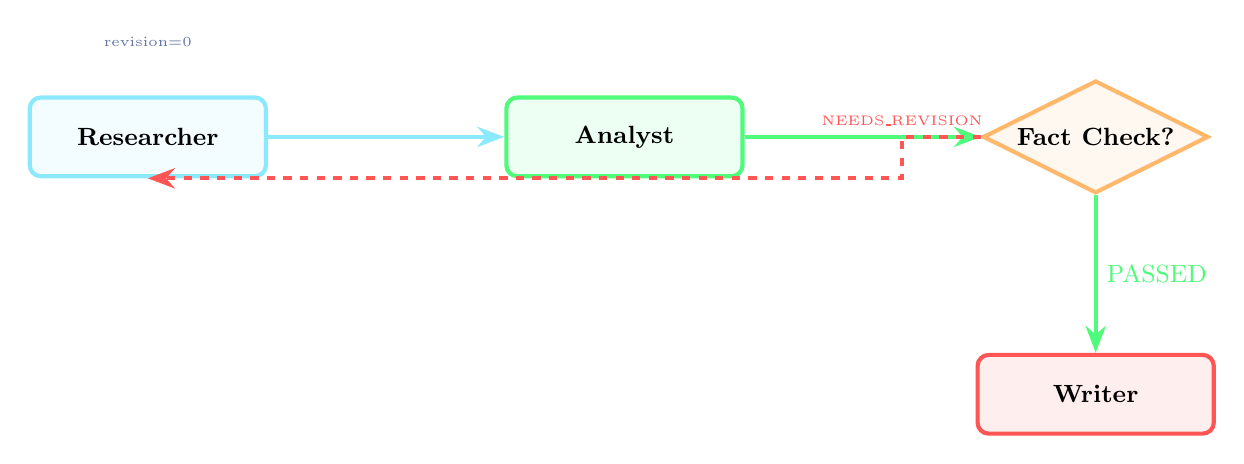
\begin{tikzpicture}[
    node distance=2cm,
    box/.style={draw=#1, rounded corners, fill=#1!10, minimum width=3cm,
                minimum height=1cm, font=\small\bfseries, line width=1.5pt},
    decision/.style={draw=accentorange, diamond, aspect=2, fill=accentorange!10,
                     font=\small\bfseries, line width=1.5pt, inner sep=2pt}
]
    \node[box=accentblue] (res) {Researcher};
    \node[box=accentgreen, right=3cm of res] (ana) {Analyst};
    \node[decision, right=3cm of ana] (fc) {Fact Check?};
    \node[box=accentred, below=2cm of fc] (wr) {Writer};
    \node[above=0.5cm of res, font=\tiny\color{comment}] {revision=0};

    \draw[-{Stealth}, accentblue, line width=1.5pt] (res) -- (ana);
    \draw[-{Stealth}, accentgreen, line width=1.5pt] (ana) -- (fc);
    \draw[-{Stealth}, accentgreen, line width=1.5pt] (fc) -- node[right, font=\small] {PASSED} (wr);
    \draw[-{Stealth}, accentred, line width=1.5pt, dashed]
        (fc.west) -- ++(-1,0) node[above, font=\tiny\color{accentred}] {NEEDS\_REVISION}
        |- (res.south);
\end{tikzpicture}
\end{center}

\textbf{Flow:}
\begin{enumerate}
\item Round 1: Researcher searches $\rightarrow$ Analyst analyzes $\rightarrow$ Fact Checker says ``NEEDS\_REVISION'' $\rightarrow$ revision\_count becomes 1
\item Round 2: Researcher searches again (with feedback) $\rightarrow$ Analyst re-analyzes $\rightarrow$ Fact Checker says ``NEEDS\_REVISION'' again $\rightarrow$ BUT revision\_count(1) $<$ MAX\_REVISIONS(2) toh revision\_count becomes 2
\item Round 3: Agar phir NEEDS\_REVISION aaya --- lekin ab revision\_count(2) $\geq$ MAX\_REVISIONS(2) toh \texttt{passed = True} force ho jata hai $\rightarrow$ Writer ko bhej do
\end{enumerate}

\textbf{Kyun max 2 revisions?} Kyunki:
\begin{itemize}
\item Har revision mein 3 Tavily API calls + LLM calls hoti hain (cost + time)
\item Infinite loop ka risk --- agar LLM hamesha ``NEEDS\_REVISION'' kehta rahe
\item 2 rounds mein 90\%+ claims usually verify ho jaate hain
\end{itemize}
\end{conceptbox}


% ######################################################################
%  SECTION 7: WRITER AGENT
% ######################################################################
\newpage
\section{Writer Agent --- \texttt{agents/writer.py}}

\begin{storybox}
Writer agent ek \textbf{professional report writer} hai. Uske paas aata hai:
\begin{itemize}
\item Verified analysis (Analyst se)
\item Fact check notes (Fact Checker se)
\item Raw research data (Researcher se)
\item RAG document context (uploaded PDFs se)
\end{itemize}
Aur woh isse ek \textbf{polished markdown report} mein convert karta hai with:
\begin{itemize}
\item Executive Summary
\item Key Findings (with inline citations [1], [2])
\item Detailed Analysis
\item Contradictions \& Debates
\item Conclusion
\item Sources Bibliography
\end{itemize}
Plus --- report complete hone ke baad, Writer \textbf{session ko ChromaDB mein store} karta hai for future memory!
\end{storybox}

\subsection{Complete Code}

\begin{lstlisting}[style=pythonstyle, title={\color{accentgreen}\faIcon{file} agents/writer.py --- Full Code (135 lines)}]
"""
Writer Agent
--------------
Synthesizes verified analysis and research data into a
polished, well-structured markdown report with inline
citations, executive summary, and sources bibliography.
"""

from langchain_groq import ChatGroq
from langchain_core.messages import (
    SystemMessage, HumanMessage
)
from config.settings import MODEL_NAME
from state.schema import ResearchState

llm = ChatGroq(model=MODEL_NAME, temperature=0.3) # Line 15

WRITER_SYSTEM_PROMPT = """You are an expert research
report writer. You produce polished, professional
research reports in markdown format.

Your report MUST include these sections:
1. **Executive Summary** -- 2-3 paragraph overview
2. **Key Findings** -- Bulleted list with citations
3. **Detailed Analysis** -- Deep dive into themes
4. **Contradictions & Debates** -- Conflicting info
5. **Conclusion** -- Synthesis and open questions
6. **Sources** -- Numbered list of URLs

GUIDELINES:
- Use inline citations like [1], [2]
- Clear, professional tone for business audience
- Use markdown: headers, bullets, bold, blockquotes
- Include specific data points and statistics
- Report should be 800-1500 words
- Do NOT fabricate information"""               # Line 34


def writer_node(state: ResearchState) -> dict:   # Line 37
    """Writer agent node."""
    topic = state["topic"]
    analysis = state.get("analysis", "")
    fact_check_result = state.get("fact_check_result", "")
    research_data = state.get("research_data", [])
    rag_context = state.get("rag_context", [])

    # Extract source URLs for bibliography
    sources = []                                  # Line 45
    for item in research_data:
        if "[Source:" in item:
            try:
                url = item.split("[Source: ")[1] \
                          .split("]")[0]
                if url not in sources \
                   and url != "Unknown source":
                    sources.append(url)
            except (IndexError, ValueError):
                pass

    # Extract RAG document sources
    doc_sources = []                              # Line 57
    for item in rag_context:
        if "[RAG Source:" in item:
            try:
                src = item.split("[RAG Source: ")[1] \
                          .split("]")[0]
                if src not in doc_sources:
                    doc_sources.append(src)
            except (IndexError, ValueError):
                pass

    # Build combined sources list
    all_sources = []
    for url in sources:
        all_sources.append(url)
    for src in doc_sources:
        all_sources.append(f"(DOC) {src}")

    sources_text = "\n".join(
        f"[{i+1}] {src}"
        for i, src in enumerate(all_sources)
    )
    compiled_data = "\n\n".join(
        research_data[:10]  # Cap to avoid token limits
    )

    # Add RAG context section
    rag_section = ""
    if rag_context:
        compiled_rag = "\n\n".join(rag_context[:5])
        rag_section = f"""

DOCUMENT CONTEXT (from uploaded files & past research):
{compiled_rag}"""

    prompt = f"""Write a comprehensive research report
on: "{topic}"

STRUCTURED ANALYSIS:
{analysis}

FACT-CHECK NOTES:
{fact_check_result}

RAW RESEARCH DATA:
{compiled_data}
{rag_section}

AVAILABLE SOURCES FOR CITATION:
{sources_text}

Write the full report using source numbers [1], [2].
Include both web and document sources."""

    response = llm.invoke([                       # Line 104
        SystemMessage(content=WRITER_SYSTEM_PROMPT),
        HumanMessage(content=prompt),
    ])

    report = response.content                     # Line 108

    # -- Store session in ChromaDB for memory -----
    try:                                          # Line 111
        from rag.vector_store import (
            store_research_session
        )
        chunks_stored = store_research_session(
            topic, research_data, report
        )
        memory_msg = (f"Stored {chunks_stored} "
                      f"chunks to research memory")
    except Exception:
        memory_msg = "Memory storage skipped"

    return {                                      # Line 120
        "final_report": report,
        "messages": [
            "Writer: Final report completed",
            memory_msg,
        ],
        "current_agent": "writer",
    }
\end{lstlisting}

\begin{codestorybox}
\textbf{Key Insights:}

\textbf{Line 15: \texttt{temperature=0.3}} --- Writer ko ``well-written'' output chahiye --- thodi creativity zaroori hai for good prose. But zyada creativity $=$ hallucination risk. 0.3 is the sweet spot.

\textbf{Lines 45-55: Source URL Extraction} --- Research data mein har result \texttt{[Source: https://...]} format mein hota hai. Writer ye URLs extract karke bibliography banata hai. String parsing use karta hai:
\begin{lstlisting}[style=pythonstyle]
# Example data item:
"[Source: https://example.com/article]\nAI is growing"

# Parsing:
url = item.split("[Source: ")[1].split("]")[0]
# Step 1: "[Source: ".split => "https://example.com/article]\nAI..."
# Step 2: "]".split => "https://example.com/article"
\end{lstlisting}

\textbf{Lines 73-74: \texttt{research\_data[:10]}} --- Ye token limit ke liye hai. LLM mein ek limit hoti hai kitna text ek baar mein process ho sakta hai (context window). Agar 50 results bhejenge toh overflow ho jayega. Top 10 sufficient hain.

\textbf{Lines 111-118: Memory Storage} --- \textbf{Ye is project ka ``learning'' feature hai.} Har successful research session ka data ChromaDB mein store hota hai. Matlab:
\begin{itemize}
\item Aaj ``AI Ethics'' research kiya $\rightarrow$ stored in \texttt{past\_research}
\item Kal ``AI Regulations'' research karo $\rightarrow$ Researcher automatically ``AI Ethics'' ka context bhi dhundh lega
\item System time ke saath \textbf{smarter} hota jaata hai!
\end{itemize}
\end{codestorybox}

\begin{memorybox}
\textbf{Temperature Cheat Sheet:}
\begin{center}
\begin{tabular}{|c|c|l|}
\hline
\rowcolor{accentpurple!15}
\textbf{Agent} & \textbf{Temp} & \textbf{Reason} \\
\hline
Researcher & 0.0 & Deterministic queries \\
Analyst & 0.1 & Controlled creativity \\
Fact Checker & 0.0 & Strict factual matching \\
Writer & 0.3 & Good prose quality \\
\hline
\end{tabular}
\end{center}
``\textbf{Jitna factual kaam, utna kam temperature. Jitna creative kaam, utna zyada.}''
\end{memorybox}


% ######################################################################
%  SECTION 8: LANGGRAPH WORKFLOW
% ######################################################################
\newpage
\section{LangGraph Workflow --- \texttt{graph/workflow.py}}

\begin{storybox}
Ab humne 4 agents bana liye. Lekin ye akele kaam nahi kar sakte --- inhe ek \textbf{assembly line} mein lagana padega. LangGraph ye kaam karta hai --- ye agents ko ek \textbf{directed graph} mein wire karta hai jahan:
\begin{itemize}
\item Nodes = Agents (functions)
\item Edges = Data flow connections
\item Conditional Edges = Decision points (``agar pass toh Writer, fail toh Researcher'')
\end{itemize}
Socho ek \textbf{factory assembly line} --- car ka chassis pehle banta hai, phir engine lagta hai, phir quality check, phir painting. Agar quality check fail ho toh wapas engine section mein bhejo.
\end{storybox}

\subsection{Complete Code}

\begin{lstlisting}[style=pythonstyle, title={\color{accentgreen}\faIcon{file} graph/workflow.py --- Full Code (78 lines)}]
"""
LangGraph Workflow
-------------------
Wires the 4 agents into a StateGraph pipeline with a
conditional feedback loop:
  Researcher -> Analyst -> Fact-Checker -> Writer
where Fact-Checker can route back to Researcher.
"""

from langgraph.graph import StateGraph, END       # Line 10
from state.schema import ResearchState            # Line 12
from agents.researcher import researcher_node     # Line 13
from agents.analyst import analyst_node           # Line 14
from agents.fact_checker import fact_checker_node  # Line 15
from agents.writer import writer_node             # Line 16


def should_continue(state: ResearchState) -> str: # Line 19
    """
    Conditional edge after the Fact-Checker node.

    Routes to:
    - "writer"     -> if fact-check passed
    - "researcher" -> if fact-check failed
    """
    if state.get("fact_check_passed", True):       # Line 27
        return "writer"
    else:
        return "researcher"                        # Line 30


def build_graph() -> StateGraph:                   # Line 33
    """
    Build and compile the research orchestrator graph.
    Pipeline: researcher -> analyst -> fact_checker
              -> (writer | researcher)
    """
    # Create graph with shared state schema
    workflow = StateGraph(ResearchState)            # Line 40

    # -- Register nodes --------------------------------
    workflow.add_node("researcher", researcher_node) # 43
    workflow.add_node("analyst", analyst_node)        # 44
    workflow.add_node("fact_checker",
                      fact_checker_node)              # 45
    workflow.add_node("writer", writer_node)          # 46

    # -- Define edges (pipeline flow) ------------------
    workflow.set_entry_point("researcher")           # Line 49

    # Sequential edges
    workflow.add_edge("researcher", "analyst")       # Line 52
    workflow.add_edge("analyst", "fact_checker")     # Line 53

    # Conditional edge: fact_checker -> writer OR
    #                   fact_checker -> researcher
    workflow.add_conditional_edges(                   # Line 56
        "fact_checker",         # Source node
        should_continue,        # Decision function
        {                       # Route map
            "writer": "writer",
            "researcher": "researcher",
        },
    )

    # Terminal edge: writer -> END
    workflow.add_edge("writer", END)                 # Line 66

    # -- Compile and return ----------------------------
    graph = workflow.compile()                        # Line 69
    return graph


# Pre-built graph instance for import
research_graph = build_graph()                       # Line 74
\end{lstlisting}

\begin{codestorybox}
\textbf{Every Line Matters:}

\textbf{Line 10: \texttt{from langgraph.graph import StateGraph, END}}
\begin{itemize}
\item \texttt{StateGraph} --- Ye class hai jo graph banati hai. Isko state schema pass karte ho (\texttt{ResearchState}), aur ye ensure karta hai ki har node correct types return kare.
\item \texttt{END} --- Ye ek special sentinel node hai. Jab koi node END se connect hota hai, matlab ``pipeline yahan khatam.''
\end{itemize}

\textbf{Line 19-30: \texttt{should\_continue()} --- The Decision Function}

Ye function \textbf{conditional routing} implement karta hai. LangGraph is function ko Fact Checker ke baad call karta hai:
\begin{lstlisting}[style=pythonstyle]
def should_continue(state: ResearchState) -> str:
    if state.get("fact_check_passed", True):
        return "writer"      # Sab verified -> Writer
    else:
        return "researcher"  # Issues found -> Researcher
\end{lstlisting}

Note: \texttt{state.get("fact\_check\_passed", True)} --- default \texttt{True}. Matlab agar key missing ho (edge case), toh assume ``passed.'' Ye \textbf{fail-safe} design hai.

\textbf{Line 40: \texttt{StateGraph(ResearchState)}} --- Graph create karte waqt schema pass karte hain. Ye batata hai LangGraph ko ki ``state ka structure ye hai, isko validate karo.''

\textbf{Lines 43-46: Node Registration} --- \texttt{add\_node(name, function)} se har agent register hota hai. Name string hona chahiye --- ye name baad mein edges mein use hota hai.

\textbf{Line 49: \texttt{set\_entry\_point("researcher")}} --- Pipeline kahan se start hogi. Hamesha Researcher pehle.

\textbf{Lines 52-53: Sequential Edges} --- \texttt{add\_edge(A, B)} matlab ``A ke baad B chalao.'' Simple, unidirectional flow.

\textbf{Lines 56-63: Conditional Edges} --- Ye sabse powerful feature hai:
\begin{lstlisting}[style=pythonstyle]
workflow.add_conditional_edges(
    "fact_checker",      # After this node...
    should_continue,     # ...call this function...
    {                    # ...and route based on return:
        "writer": "writer",       # "writer" -> writer node
        "researcher": "researcher", # "researcher" -> researcher
    },
)
\end{lstlisting}

Route map ka format: \texttt{\{function\_return\_value: node\_name\}}

\textbf{Line 66: \texttt{add\_edge("writer", END)}} --- Writer ke baad pipeline khatam.

\textbf{Line 69: \texttt{workflow.compile()}} --- Graph ko ``freeze'' karta hai. Compile ke baad nodes/edges add nahi kar sakte. Ye compiled graph ab \texttt{.invoke()} ya \texttt{.stream()} se run ho sakta hai.

\textbf{Line 74: Module-level instance} --- \texttt{research\_graph = build\_graph()} module load hote hi graph ban jaata hai. \texttt{from graph.workflow import research\_graph} se koi bhi file isko use kar sakti hai.
\end{codestorybox}

\begin{conceptbox}[title={\faIcon{brain} ~LangGraph Internals --- How the Engine Works}]
Jab tum \texttt{research\_graph.invoke(initial\_state)} call karte ho:

\begin{enumerate}[label=\textcolor{accentpurple}{Step \arabic*:}]
\item \textbf{Entry Point Check:} LangGraph entry point dhundhta hai $\rightarrow$ ``researcher''
\item \textbf{Node Execution:} \texttt{researcher\_node(state)} call hota hai. Ye ek dict return karta hai.
\item \textbf{State Merge:} Return dict ko current state mein merge karta hai. \texttt{Annotated} fields ke liye reducer use hota hai (\texttt{operator.add}), baaki overwrite.
\item \textbf{Edge Resolution:} ``researcher'' ke outgoing edges check karta hai $\rightarrow$ ``analyst'' milta hai
\item \textbf{Repeat:} Analyst execute $\rightarrow$ merge $\rightarrow$ Fact Checker pe jaao
\item \textbf{Conditional Edge:} Fact Checker ke baad \texttt{should\_continue(state)} call hota hai
\item \textbf{Routing:} Agar ``writer'' return hua $\rightarrow$ Writer execute karo. Agar ``researcher'' $\rightarrow$ wapas Step 2 pe jaao
\item \textbf{Terminal:} Writer ke baad END milta hai $\rightarrow$ Final state return
\end{enumerate}

\textbf{recursion\_limit:} \texttt{\{``recursion\_limit'': 25\}} ka matlab hai max 25 node executions allowed hain. Agar feedback loop 25 se zyada baar chale (bug!), toh LangGraph exception throw karega.
\end{conceptbox}

\begin{interviewbox}[title={\faIcon{user-tie} ~Q: \texttt{.invoke()} vs \texttt{.stream()} mein kya fark hai?}]
\textbf{A:}
\begin{itemize}
\item \texttt{.invoke(state)} --- Pura graph run karo aur final state return karo. Synchronous call. Simple use case ke liye.
\item \texttt{.stream(state)} --- Har node ke baad intermediate result yield karo. Generator return karta hai. UI ke liye perfect --- real-time progress dikhao.
\end{itemize}

\textbf{Code comparison:}
\begin{lstlisting}[style=pythonstyle]
# invoke -- sab ek baar mein
result = graph.invoke(initial_state)
print(result["final_report"])

# stream -- step by step
for event in graph.stream(initial_state):
    for node_name, output in event.items():
        print(f"{node_name} completed!")
        # UI update karo
\end{lstlisting}

Humara \texttt{app.py} mein \texttt{.stream()} use hota hai taki Streamlit UI mein real-time agent progress dikhe.
\end{interviewbox}


% ######################################################################
%  SECTION 9: RAG SYSTEM DEEP DIVE
% ######################################################################
\newpage
\section{RAG System --- \texttt{rag/vector\_store.py}}

\begin{storybox}
RAG (Retrieval Augmented Generation) ko samajhne ke liye ek example lo:

Tum ek student ho jo exam ki tayyari kar raha hai. Tumhare paas do options hain:
\begin{enumerate}
\item \textbf{Bina notes:} Sab yaad se likho (LLM alone --- hallucination risk)
\item \textbf{Notes ke saath:} Pehle relevant notes dhundho, phir unke basis pe likho (LLM + RAG --- accurate!)
\end{enumerate}

RAG exactly yahi karta hai:
\begin{enumerate}
\item \textbf{R}etrieval --- Relevant documents dhundho (semantic search)
\item \textbf{A}ugmented --- Retrieved context ko LLM ke prompt mein add karo
\item \textbf{G}eneration --- LLM augmented context ke basis pe answer generate kare
\end{enumerate}

Is project mein RAG do tarike se use hota hai:
\begin{itemize}
\item \textbf{Document RAG:} User PDF upload kare $\rightarrow$ chunks mein todo $\rightarrow$ ChromaDB mein store $\rightarrow$ research ke waqt search
\item \textbf{Memory RAG:} Past research sessions store $\rightarrow$ future research mein context provide
\end{itemize}
\end{storybox}

\subsection{Embedding Mathematics}

\begin{mathbox}
\textbf{Embedding kya hai?}

Text ko numbers (vectors) mein convert karna. Har word/sentence ko ek high-dimensional vector mein map karna.

\textbf{Example:}
\begin{align}
\text{``AI is powerful''} &\rightarrow [0.12, -0.34, 0.56, \ldots, 0.78] \quad \text{(384 dimensions)} \\
\text{``Machine learning rocks''} &\rightarrow [0.11, -0.32, 0.55, \ldots, 0.80]  \\
\text{``I like pizza''} &\rightarrow [0.89, 0.12, -0.67, \ldots, -0.45]
\end{align}

Notice: ``AI is powerful'' aur ``Machine learning rocks'' ke vectors \textbf{similar} hain (close numbers), lekin ``I like pizza'' ka vector \textbf{bahut different} hai. Ye \textbf{semantic similarity} hai!

\textbf{Cosine Similarity Formula:}
\[
\text{similarity}(\vec{a}, \vec{b}) = \frac{\vec{a} \cdot \vec{b}}{||\vec{a}|| \times ||\vec{b}||} = \frac{\sum_{i=1}^{n} a_i \cdot b_i}{\sqrt{\sum_{i=1}^{n} a_i^2} \times \sqrt{\sum_{i=1}^{n} b_i^2}}
\]

\begin{itemize}
\item Result range: $[-1, 1]$ (normalized vectors ke liye $[0, 1]$)
\item $1.0$ = identical meaning
\item $0.0$ = no relation
\item Close to $1.0$ = semantically similar
\end{itemize}

\textbf{Humara model} \texttt{all-MiniLM-L6-v2}:
\begin{itemize}
\item Output dimension: 384 (har text $\rightarrow$ 384-dimensional vector)
\item Model size: $\sim$80 MB (small, fast, free)
\item Training: 1 billion+ sentence pairs pe trained
\item Speed: $\sim$14,000 sentences/second on CPU
\end{itemize}
\end{mathbox}

\subsection{Chunking Strategy}

\begin{conceptbox}[title={\faIcon{brain} ~Kyun Chunking Zaroori Hai?}]
Ek 100-page PDF ko directly vector store mein nahi daal sakte. Kyun?
\begin{enumerate}
\item \textbf{Embedding models ka limit:} all-MiniLM-L6-v2 max 256 tokens process karta hai. Isse zyada text mein information loss hota hai.
\item \textbf{Retrieval precision:} Agar pura document ek vector hai, toh search ``approximate'' hogi. Chhote chunks se precise matching hoti hai.
\item \textbf{LLM context window:} Retrieved chunks LLM ke prompt mein jaate hain. Agar chunk bahut bada ho toh prompt overflow ho jayega.
\end{enumerate}

\textbf{Humara approach: RecursiveCharacterTextSplitter}
\begin{lstlisting}[style=pythonstyle]
text_splitter = RecursiveCharacterTextSplitter(
    chunk_size=1000,        # Max 1000 characters per chunk
    chunk_overlap=200,      # 200 chars overlap between chunks
    separators=["\n\n", "\n", ". ", " ", ""],
)
\end{lstlisting}

\textbf{Kaise kaam karta hai?}
\begin{enumerate}
\item Pehle \texttt{"\textbackslash n\textbackslash n"} (double newline, i.e., paragraph break) pe split karne ki koshish
\item Agar chunk 1000 se bada hai, toh \texttt{"\textbackslash n"} (single newline) pe try
\item Phir \texttt{". "} (sentence boundary) pe try
\item Phir \texttt{" "} (word boundary)
\item Last resort: character level split
\end{enumerate}

\textbf{Overlap kyun?} Socho ek sentence do chunks ke beech split ho gaya --- context kho jayega. 200 chars overlap se ek chunk ka end doosre chunk ke start mein include hota hai. Ye ``sliding window'' approach hai.
\end{conceptbox}

\subsection{Complete Code}

\begin{lstlisting}[style=pythonstyle, title={\color{accentgreen}\faIcon{file} rag/vector\_store.py --- Key Functions}]
"""
RAG Vector Store Manager
--------------------------
Handles PDF ingestion, chunking, embedding, and retrieval
using ChromaDB (persistent) + HuggingFace embeddings.
"""

import os
import hashlib
from typing import Optional

from langchain_huggingface import HuggingFaceEmbeddings
from langchain_chroma import Chroma
from langchain_community.document_loaders import PyPDFLoader
from langchain_text_splitters import (
    RecursiveCharacterTextSplitter
)
from langchain_core.documents import Document

from config.settings import (
    CHROMA_PERSIST_DIR, EMBEDDING_MODEL,
    CHUNK_SIZE, CHUNK_OVERLAP,
)


# -- Embedding Model (singleton) ----------------------
_embeddings = None                                # Line 28

def get_embeddings() -> HuggingFaceEmbeddings:    # Line 30
    """Get or create the HuggingFace embedding model."""
    global _embeddings
    if _embeddings is None:                        # Line 33
        _embeddings = HuggingFaceEmbeddings(
            model_name=EMBEDDING_MODEL,
            model_kwargs={"device": "cpu"},
            encode_kwargs={"normalize_embeddings": True},
        )
    return _embeddings
\end{lstlisting}

\begin{codestorybox}
\textbf{Singleton Pattern Explained:}

\texttt{\_embeddings = None} (module-level variable). Pehli baar \texttt{get\_embeddings()} call hone pe model load hota hai (slow --- $\sim$2-3 seconds). Uske baad har call pe cached instance return hota hai (instant).

\textbf{Kyun Singleton?}
\begin{itemize}
\item Model load karna expensive hai (memory + time)
\item Ek hi model multiple baar load karna wasteful hai
\item \texttt{global \_embeddings} se function ke bahar ki variable modify kar sakte hain
\end{itemize}

\textbf{\texttt{normalize\_embeddings=True}} --- Vectors ko unit length pe normalize karta hai. Iska fayda: cosine similarity calculate karna faster ho jata hai (denominator 1 ho jata hai toh sirf dot product chahiye).
\end{codestorybox}

\begin{lstlisting}[style=pythonstyle, title={\color{accentgreen}\faIcon{file} Vector Store Access}]
def get_vectorstore(collection_name="research_docs"):
    """Get or create a persistent ChromaDB store."""
    os.makedirs(CHROMA_PERSIST_DIR, exist_ok=True)
    return Chroma(
        collection_name=collection_name,
        embedding_function=get_embeddings(),
        persist_directory=CHROMA_PERSIST_DIR,
    )
\end{lstlisting}

\begin{codestorybox}
\textbf{\texttt{os.makedirs()} with \texttt{exist\_ok=True}} --- Directory banao agar nahi hai. \texttt{exist\_ok=True} se agar already hai toh error nahi aayega.

\textbf{\texttt{persist\_directory}} --- ChromaDB ka data disk pe save hota hai is directory mein. Matlab app restart hone pe bhi data rehta hai. Bina iske sab memory mein hota --- app band karo, data gayab.

\textbf{Two Collections:}
\begin{enumerate}
\item \texttt{"research\_docs"} --- User uploaded PDFs ke chunks
\item \texttt{"past\_research"} --- Previous research sessions ka data
\end{enumerate}
Ye ek database mein do tables jaisa hai --- alag-alag data, same engine.
\end{codestorybox}

\begin{lstlisting}[style=pythonstyle, title={\color{accentgreen}\faIcon{file} PDF Ingestion Function}]
def ingest_documents(file_paths: list[str]) -> dict:
    """Load PDFs, chunk, embed, store in ChromaDB."""
    text_splitter = RecursiveCharacterTextSplitter(
        chunk_size=CHUNK_SIZE,
        chunk_overlap=CHUNK_OVERLAP,
        separators=["\n\n", "\n", ". ", " ", ""],
    )

    all_chunks = []
    files_processed = []

    for file_path in file_paths:
        try:
            loader = PyPDFLoader(file_path)
            docs = loader.load()     # List[Document]

            # Add file metadata
            file_name = os.path.basename(file_path)
            for doc in docs:
                doc.metadata["source_file"] = file_name

            # Split into chunks
            chunks = text_splitter.split_documents(docs)
            all_chunks.extend(chunks)
            files_processed.append(file_name)
        except Exception as e:
            files_processed.append(
                f"{os.path.basename(file_path)} (ERROR: {e})"
            )

    if all_chunks:
        # Generate unique IDs (content hash = no dupes)
        ids = []
        for chunk in all_chunks:
            content_hash = hashlib.md5(
                chunk.page_content.encode()
            ).hexdigest()
            ids.append(content_hash)

        vectorstore = get_vectorstore("research_docs")
        vectorstore.add_documents(
            documents=all_chunks, ids=ids
        )

    return {
        "chunks_added": len(all_chunks),
        "files_processed": files_processed,
    }
\end{lstlisting}

\begin{codestorybox}
\textbf{Ingestion Pipeline Step-by-Step:}

\begin{center}
\begin{tikzpicture}[
    node distance=0.8cm,
    step/.style={draw=accentblue, rounded corners=5pt, fill=accentblue!10,
                 text width=4cm, align=center, minimum height=0.8cm,
                 font=\small, line width=1pt},
    arr/.style={-{Stealth[length=3mm]}, accentpurple, line width=1.5pt}
]
    \node[step] (s1) {PDF File};
    \node[step, below=of s1] (s2) {PyPDFLoader.load()};
    \node[step, below=of s2] (s3) {List[Document]\\(1 doc per page)};
    \node[step, below=of s3] (s4) {TextSplitter.split()};
    \node[step, below=of s4] (s5) {List[Document]\\(chunks of 1000 chars)};
    \node[step, below=of s5] (s6) {HuggingFace Embed};
    \node[step, below=of s6] (s7) {ChromaDB Store};

    \draw[arr] (s1) -- (s2);
    \draw[arr] (s2) -- (s3);
    \draw[arr] (s3) -- (s4);
    \draw[arr] (s4) -- (s5);
    \draw[arr] (s5) -- (s6);
    \draw[arr] (s6) -- (s7);
\end{tikzpicture}
\end{center}

\textbf{MD5 Hash for Deduplication:}
\begin{lstlisting}[style=pythonstyle]
content_hash = hashlib.md5(
    chunk.page_content.encode()
).hexdigest()
\end{lstlisting}
Same content ka same hash hoga. Toh agar user same PDF dobara upload kare, toh duplicate chunks nahi banenge --- ChromaDB same ID wale documents overwrite kar deta hai.
\end{codestorybox}

\begin{lstlisting}[style=pythonstyle, title={\color{accentgreen}\faIcon{file} Semantic Retrieval}]
def retrieve_context(
    query: str,
    collection_name: str = "research_docs",
    k: int = 5,
) -> list[str]:
    """Retrieve most relevant chunks from ChromaDB."""
    vectorstore = get_vectorstore(collection_name)

    try:
        results = vectorstore.similarity_search(
            query, k=k
        )
    except Exception:
        return []

    if not results:
        return []

    formatted = []
    for doc in results:
        source = doc.metadata.get(
            "source_file",
            doc.metadata.get("source", "Unknown")
        )
        page = doc.metadata.get("page", "")
        source_info = f"[RAG Source: {source}"
        if page != "":
            source_info += f", Page {int(page) + 1}"
        source_info += "]"
        formatted.append(
            f"{source_info}\n{doc.page_content}"
        )

    return formatted
\end{lstlisting}

\begin{codestorybox}
\textbf{Retrieval Process:}
\begin{enumerate}
\item User query aati hai: ``What are the effects of AI on healthcare?''
\item Query ko embed kiya jaata hai $\rightarrow$ 384-dimensional vector
\item ChromaDB mein stored vectors ke saath cosine similarity calculate hota hai
\item Top-k (default 5) most similar chunks return hote hain
\item Har chunk ke saath source metadata attach hota hai (filename, page number)
\end{enumerate}

\textbf{Note:} \texttt{page + 1} kyunki PyPDFLoader 0-indexed pages return karta hai, lekin humans 1-indexed count karte hain.
\end{codestorybox}

\begin{lstlisting}[style=pythonstyle, title={\color{accentgreen}\faIcon{file} Research Session Memory}]
def store_research_session(
    topic: str,
    research_data: list[str],
    report: str,
) -> int:
    """Store completed session for future retrieval."""
    text_splitter = RecursiveCharacterTextSplitter(
        chunk_size=CHUNK_SIZE,
        chunk_overlap=CHUNK_OVERLAP,
    )

    documents = []

    # Store the final report
    if report:
        report_doc = Document(
            page_content=report,
            metadata={
                "source": f"Past Research: {topic}",
                "type": "report"
            },
        )
        documents.append(report_doc)

    # Store key research data (cap at 10)
    for i, data in enumerate(research_data[:10]):
        doc = Document(
            page_content=data,
            metadata={
                "source": f"Past Research: {topic}",
                "type": "research_data",
                "index": i,
            },
        )
        documents.append(doc)

    if documents:
        chunks = text_splitter.split_documents(documents)
        ids = [
            hashlib.md5(
                f"{topic}_{i}_{c.page_content[:50]}"
                .encode()
            ).hexdigest()
            for i, c in enumerate(chunks)
        ]

        vectorstore = get_vectorstore("past_research")
        vectorstore.add_documents(
            documents=chunks, ids=ids
        )
        return len(chunks)

    return 0
\end{lstlisting}

\begin{codestorybox}
\textbf{Memory System Design:}

Ye function Writer agent ke end mein call hota hai. Har successful research session ka:
\begin{enumerate}
\item \textbf{Final report} store hota hai (high-quality summarized content)
\item \textbf{Raw research data} ke top 10 results store hote hain (source material)
\end{enumerate}

ID generation mein \texttt{topic} bhi include hai: \texttt{f"\{topic\}\_\{i\}\_\{content[:50]\}"}. Ye ensure karta hai ki same topic pe repeat research karne pe puraane chunks overwrite hon (same ID $\rightarrow$ overwrite).

\textbf{Future Impact:} Jab Researcher agent next time koi related topic search karega, \texttt{retrieve\_context("past\_research")} call se ye stored chunks automatic mil jayenge!
\end{codestorybox}

\begin{lstlisting}[style=pythonstyle, title={\color{accentgreen}\faIcon{file} Utility Functions}]
def get_collection_stats() -> dict:
    """Get document counts for all collections."""
    stats = {}
    for name in ["research_docs", "past_research"]:
        try:
            vs = get_vectorstore(name)
            collection = vs._collection
            stats[name] = collection.count()
        except Exception:
            stats[name] = 0
    return stats


def clear_collection(
    collection_name: str = "research_docs"
) -> bool:
    """Clear all documents from a collection."""
    try:
        vs = get_vectorstore(collection_name)
        collection = vs._collection
        all_ids = collection.get()["ids"]
        if all_ids:
            collection.delete(ids=all_ids)
        return True
    except Exception:
        return False
\end{lstlisting}

\begin{codestorybox}
\textbf{\texttt{vs.\_collection}} --- Ye ChromaDB ka internal collection object access karta hai. Underscore prefix (\texttt{\_}) ka matlab hai ``private variable'' --- normally directly access nahi karna chahiye, lekin LangChain wrapper mein \texttt{.count()} method nahi hai, toh yahi option hai.

\textbf{\texttt{clear\_collection}} --- Pehle sabke IDs get karo, phir delete karo. ChromaDB mein bulk delete ke liye IDs list dena padta hai --- ``delete all'' jaise shortcut nahi hai.
\end{codestorybox}


% ######################################################################
%  SECTION 10: MCP SERVER
% ######################################################################
\newpage
\section{MCP Server --- \texttt{mcp\_server.py}}

\begin{storybox}
\textbf{MCP (Model Context Protocol)} ko samjhne ke liye socho:

Tumhare paas ek amazing research system hai (humara orchestrator). Ab tum chahte ho ki \textbf{Claude Desktop} ya \textbf{Cursor IDE} directly isse use kar sake --- bina Streamlit UI open kiye.

MCP exactly ye karta hai --- ye ek \textbf{standard protocol} hai (jaise HTTP web ke liye hai) jo AI tools ko ek dusre se baat karne deta hai. Humara MCP server 5 ``tools'' expose karta hai jo koi bhi MCP client call kar sakta hai.

\textbf{Analogy:} USB port socho. Koi bhi device (mouse, keyboard, pen drive) USB mein lag sakta hai kyunki standard hai. MCP wahi hai AI tools ke liye --- ek universal plug.
\end{storybox}

\subsection{MCP Architecture}

\begin{center}
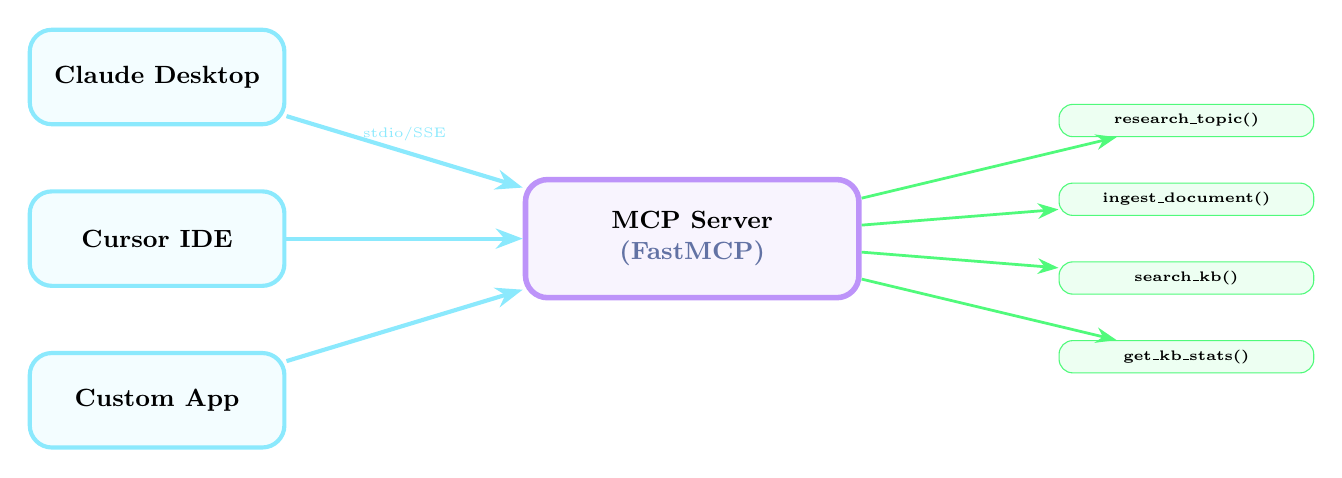
\begin{tikzpicture}[
    node distance=1.5cm and 2.5cm,
    client/.style={draw=accentblue, rounded corners=8pt, fill=accentblue!10,
                   text width=3cm, align=center, minimum height=1.2cm,
                   font=\small\bfseries, line width=1.5pt},
    server/.style={draw=accentpurple, rounded corners=8pt, fill=accentpurple!10,
                   text width=4cm, align=center, minimum height=1.5cm,
                   font=\small\bfseries, line width=2pt},
    tool/.style={draw=accentgreen, rounded corners=5pt, fill=accentgreen!10,
                 text width=3cm, align=center, font=\tiny\bfseries},
]
    % Clients
    \node[client] (claude) {Claude Desktop};
    \node[client, below=0.8cm of claude] (cursor) {Cursor IDE};
    \node[client, below=0.8cm of cursor] (custom) {Custom App};

    % Server
    \node[server, right=3cm of cursor] (mcp) {MCP Server\\{\small\color{comment}(FastMCP)}};

    % Tools
    \node[tool, right=2.5cm of mcp, yshift=1.5cm] (t1) {research\_topic()};
    \node[tool, right=2.5cm of mcp, yshift=0.5cm] (t2) {ingest\_document()};
    \node[tool, right=2.5cm of mcp, yshift=-0.5cm] (t3) {search\_kb()};
    \node[tool, right=2.5cm of mcp, yshift=-1.5cm] (t4) {get\_kb\_stats()};

    % Connections
    \draw[-{Stealth}, accentblue, line width=1.5pt] (claude) -- (mcp) node[midway, above, font=\tiny\color{comment}] {stdio/SSE};
    \draw[-{Stealth}, accentblue, line width=1.5pt] (cursor) -- (mcp);
    \draw[-{Stealth}, accentblue, line width=1.5pt] (custom) -- (mcp);
    \draw[-{Stealth}, accentgreen, line width=1pt] (mcp) -- (t1);
    \draw[-{Stealth}, accentgreen, line width=1pt] (mcp) -- (t2);
    \draw[-{Stealth}, accentgreen, line width=1pt] (mcp) -- (t3);
    \draw[-{Stealth}, accentgreen, line width=1pt] (mcp) -- (t4);
\end{tikzpicture}
\end{center}

\subsection{Complete Code}

\begin{lstlisting}[style=pythonstyle, title={\color{accentgreen}\faIcon{file} mcp\_server.py --- Full Code (208 lines)}]
"""
MCP Server -- Research Orchestrator as a Tool
-----------------------------------------------
Exposes the multi-agent research pipeline as MCP tools.
Any MCP-compatible client can call these tools.

Usage:
    # Test with MCP Inspector
    fastmcp dev mcp_server.py

    # Run as stdio server
    python mcp_server.py
"""

import sys
import os

sys.path.insert(0, os.path.dirname(
    os.path.abspath(__file__)
))

from fastmcp import FastMCP                       # Line 18

# -- Initialize MCP Server ----------------------------
mcp = FastMCP(                                    # Line 21
    "ResearchOrchestrator",
    description=(
        "Multi-Agent Research Orchestrator -- "
        "4 AI agents collaborate to research, "
        "analyze, fact-check, and write reports."
    ),
)


# -- Tool 1: Research a Topic -------------------------
@mcp.tool()                                       # Line 31
def research_topic(topic: str) -> str:
    """
    Run the full multi-agent research pipeline.
    4 agents collaborate to produce a comprehensive,
    fact-checked, cited research report.

    Args:
        topic: The research topic or question.

    Returns:
        A polished markdown research report.
    """
    from graph.workflow import research_graph

    initial_state = {
        "topic": topic,
        "research_data": [],
        "analysis": "",
        "fact_check_result": "",
        "fact_check_passed": False,
        "revision_count": 0,
        "final_report": "",
        "rag_context": [],
        "messages": [],
        "current_agent": "",
        "error": "",
    }

    try:
        result = research_graph.invoke(
            initial_state, {"recursion_limit": 25}
        )
        report = result.get("final_report", "")
        if report:
            return report
        elif result.get("error"):
            return f"Pipeline error: {result['error']}"
        else:
            return "No report generated."
    except Exception as e:
        return f"Error: {str(e)}"


# -- Tool 2: Ingest Document --------------------------
@mcp.tool()
def ingest_document(file_path: str) -> str:
    """Ingest a PDF into the RAG knowledge base."""
    from rag.vector_store import ingest_documents

    if not os.path.exists(file_path):
        return f"Error: File not found at '{file_path}'"
    if not file_path.lower().endswith(".pdf"):
        return "Error: Only PDF files supported."

    try:
        result = ingest_documents([file_path])
        return (
            f"Ingested {result['chunks_added']} chunks"
            f" from {', '.join(result['files_processed'])}"
        )
    except Exception as e:
        return f"Error: {str(e)}"


# -- Tool 3: Search Knowledge Base --------------------
@mcp.tool()
def search_knowledge_base(
    query: str, num_results: int = 5
) -> str:
    """Search the RAG knowledge base."""
    from rag.vector_store import retrieve_context

    try:
        doc_results = retrieve_context(
            query, collection_name="research_docs",
            k=num_results
        )
        past_results = retrieve_context(
            query, collection_name="past_research",
            k=3
        )
        all_results = doc_results + past_results

        if not all_results:
            return "No relevant documents found."
        return "\n\n---\n\n".join(all_results)
    except Exception as e:
        return f"Error: {str(e)}"


# -- Tool 4: KB Stats ---------------------------------
@mcp.tool()
def get_kb_stats() -> str:
    """Get RAG knowledge base statistics."""
    from rag.vector_store import get_collection_stats

    try:
        stats = get_collection_stats()
        return (
            f"Knowledge Base Stats:\n"
            f"  Uploaded Docs: "
            f"{stats.get('research_docs', 0)} chunks\n"
            f"  Research Memory: "
            f"{stats.get('past_research', 0)} chunks"
        )
    except Exception as e:
        return f"Error: {str(e)}"


# -- Tool 5: Clear KB ---------------------------------
@mcp.tool()
def clear_knowledge_base() -> str:
    """Clear all documents and memory."""
    from rag.vector_store import clear_collection

    try:
        clear_collection("research_docs")
        clear_collection("past_research")
        return "Knowledge base cleared."
    except Exception as e:
        return f"Error: {str(e)}"


# -- Resource: Project Info ----------------------------
@mcp.resource("info://orchestrator")              # Line 153
def get_info() -> str:
    """Information about the Research Orchestrator."""
    return """
Multi-Agent Research Orchestrator v1.0

Agents:
  Researcher  -- Web search + RAG retrieval
  Analyst     -- Pattern extraction, gap analysis
  Fact Checker -- Claim verification with feedback
  Writer      -- Report synthesis with citations

Tech Stack:
  LLM: Groq (openai/gpt-oss-120b)
  Search: Tavily (advanced depth)
  Vector Store: ChromaDB (persistent)
  Embeddings: HuggingFace all-MiniLM-L6-v2
  Orchestration: LangGraph StateGraph
  UI: Streamlit
  Protocol: MCP (Model Context Protocol)
"""


# -- Run Server ----------------------------------------
if __name__ == "__main__":                         # Line 175
    mcp.run(transport="stdio")
\end{lstlisting}

\begin{codestorybox}
\textbf{MCP Concepts Explained:}

\textbf{\texttt{@mcp.tool()} Decorator:} Ye kisi bhi function ko MCP tool bana deta hai. Jab Claude Desktop ya Cursor connect karta hai, toh ye tools automatically discover ho jaate hain. Function ka docstring tool ka description ban jaata hai, aur parameters automatically schema mein convert hote hain.

\textbf{\texttt{@mcp.resource("info://orchestrator")}:} Resources read-only data hain jo client access kar sakta hai. Tools ke opposite --- tools actions perform karti hain, resources sirf information provide karti hain.

\textbf{\texttt{transport="stdio"}:} MCP do transports support karta hai:
\begin{itemize}
\item \texttt{stdio} --- Standard input/output streams se communicate. Claude Desktop aur Cursor ye use karte hain. Server ek subprocess ke roop mein run hota hai.
\item \texttt{sse} --- Server-Sent Events (HTTP-based). Web applications ke liye.
\end{itemize}

\textbf{Claude Desktop mein setup:}
\begin{lstlisting}[style=bashstyle]
# claude_desktop_config.json mein add karo:
{
  "mcpServers": {
    "research": {
      "command": "python",
      "args": ["C:/path/to/mcp_server.py"]
    }
  }
}
\end{lstlisting}
Ab Claude Desktop mein ``Research AI in healthcare'' type karo aur Claude automatically humara \texttt{research\_topic()} tool call karega!
\end{codestorybox}

\begin{interviewbox}[title={\faIcon{user-tie} ~Q: MCP vs REST API mein kya fark hai?}]
\textbf{A:}
\begin{center}
\small
\begin{tabular}{|l|p{5cm}|p{5cm}|}
\hline
\rowcolor{accentpurple!15}
& \textbf{MCP} & \textbf{REST API} \\
\hline
\textbf{Purpose} & AI tool interoperability & General web APIs \\
\hline
\textbf{Discovery} & Auto-discovery (tools, resources) & Manual (docs/Swagger) \\
\hline
\textbf{Transport} & stdio or SSE & HTTP \\
\hline
\textbf{Schema} & Function signatures auto-generate & Manually define endpoints \\
\hline
\textbf{Clients} & Claude, Cursor, etc. & Any HTTP client \\
\hline
\textbf{State} & Stateful connection & Stateless requests \\
\hline
\end{tabular}
\end{center}

MCP specifically AI-to-AI communication ke liye designed hai, jabki REST general purpose hai. MCP mein tool discovery automatic hai --- client connect hota hai aur server batata hai ``mere paas ye 5 tools hain.''
\end{interviewbox}


% ######################################################################
%  SECTION 11: STREAMLIT UI (app.py) DEEP DIVE
% ######################################################################
\newpage
\section{Streamlit UI --- \texttt{app.py} Deep Dive}

\begin{storybox}
\texttt{app.py} humari ``showroom'' hai --- ye woh jagah hai jahan user interact karta hai. Is file mein 700+ lines hain covering:
\begin{enumerate}
\item Premium CSS with glassmorphism design
\item Session state management
\item Sidebar with real-time agent status
\item RAG document upload interface
\item Research pipeline execution with streaming
\item Results display with download option
\end{enumerate}
\end{storybox}

\subsection{Page Configuration}

\begin{lstlisting}[style=pythonstyle, title={\color{accentgreen}\faIcon{file} app.py --- Page Config}]
import sys, os, time
import streamlit as st

sys.path.insert(0,
    os.path.dirname(os.path.abspath(__file__))
)

# Page Config -- MUST be first Streamlit call!
st.set_page_config(
    page_title="Multi-Agent Research Orchestrator",
    page_icon="microscope",
    layout="wide",          # Full width layout
    initial_sidebar_state="expanded",
)
\end{lstlisting}

\begin{warningbox}
\texttt{st.set\_page\_config()} \textbf{MUST be the first Streamlit command} in your script. Agar pehle koi aur \texttt{st.} call aaye (even \texttt{st.write()}), toh error aayega: ``\texttt{set\_page\_config() can only be called once and must be the first Streamlit command}.''
\end{warningbox}

\subsection{Premium CSS Design}

\begin{lstlisting}[style=cssstyle, title={\color{accentgreen}\faIcon{paint-brush} Glassmorphism CSS}]
/* Glass Card Effect */
.glass-card {
    background: rgba(255, 255, 255, 0.03);
    border: 1px solid rgba(255, 255, 255, 0.08);
    border-radius: 16px;
    padding: 1.5rem;
    margin: 1rem 0;
    backdrop-filter: blur(10px);
    -webkit-backdrop-filter: blur(10px);
    transition: all 0.3s ease;
}
.glass-card:hover {
    border-color: rgba(102, 126, 234, 0.3);
    box-shadow: 0 8px 32px rgba(102, 126, 234, 0.1);
}
\end{lstlisting}

\begin{conceptbox}[title={\faIcon{brain} ~Glassmorphism Kya Hai?}]
Glassmorphism ek modern UI design trend hai jismein elements \textbf{frosted glass} jaise dikhte hain:
\begin{itemize}
\item \texttt{rgba(255, 255, 255, 0.03)} --- Almost transparent white background (3\% opacity)
\item \texttt{backdrop-filter: blur(10px)} --- Background content ko blur karta hai glass ke peeche
\item \texttt{border: 1px solid rgba(255, 255, 255, 0.08)} --- Subtle edge glow
\end{itemize}
Ye dark theme ke saath combine karke ``premium'' feel deta hai --- Apple, Microsoft ye design use karte hain.
\end{conceptbox}

\subsection{Session State Management}

\begin{lstlisting}[style=pythonstyle, title={\color{accentgreen}\faIcon{file} Session State Initialization}]
# Session State -- Streamlit reruns script on every
# interaction, so state must be preserved externally
if "research_running" not in st.session_state:
    st.session_state.research_running = False
if "research_complete" not in st.session_state:
    st.session_state.research_complete = False
if "final_report" not in st.session_state:
    st.session_state.final_report = ""
if "agent_messages" not in st.session_state:
    st.session_state.agent_messages = []
if "agent_statuses" not in st.session_state:
    st.session_state.agent_statuses = {
        "researcher": "idle",
        "analyst": "idle",
        "fact_checker": "idle",
        "writer": "idle",
    }
if "error" not in st.session_state:
    st.session_state.error = ""
\end{lstlisting}

\begin{conceptbox}[title={\faIcon{brain} ~Streamlit Ka Execution Model}]
Streamlit ka sabse important concept samjho:

\textbf{Har interaction pe pura script re-run hota hai!}

Matlab jab user button click kare, slider move kare, ya text type kare --- Streamlit pura \texttt{app.py} top se bottom tak dobara execute karta hai. Isliye:
\begin{itemize}
\item Variables normally reset ho jaate hain (har run pe naye bante hain)
\item \texttt{st.session\_state} ek persistent dictionary hai jo runs ke beech data preserve karti hai
\item \texttt{if "key" not in st.session\_state:} --- sirf pehli baar initialize karo, baad mein skip
\end{itemize}

\textbf{Analogy:} Socho ek whiteboard hai. Har baar jab koi button dabaye, whiteboard saaf ho jaata hai aur dobara likho. \texttt{session\_state} ek separate notebook hai jisko whiteboard saaf karne se kuch nahi hota.
\end{conceptbox}

\subsection{Pipeline Execution with Streaming}

\begin{lstlisting}[style=pythonstyle, title={\color{accentgreen}\faIcon{file} app.py --- Research Pipeline Execution}]
if start_btn and topic:
    # Reset state
    st.session_state.research_running = True
    st.session_state.research_complete = False
    st.session_state.final_report = ""
    st.session_state.agent_messages = []
    st.session_state.error = ""
    st.session_state.agent_statuses = {
        "researcher": "idle", "analyst": "idle",
        "fact_checker": "idle", "writer": "idle",
    }

    try:
        from graph.workflow import research_graph
    except ValueError as e:
        st.error(f"Configuration Error: {e}")
        st.stop()  # Stop execution entirely

    # Initial state for the graph
    initial_state = {
        "topic": topic,
        "research_data": [],
        "analysis": "",
        "fact_check_result": "",
        "fact_check_passed": False,
        "revision_count": 0,
        "final_report": "",
        "rag_context": [],
        "messages": [],
        "current_agent": "",
        "error": "",
    }

    # Stream the graph execution
    status_container = st.empty()
    progress_bar = st.progress(0)

    try:
        step_count = 0
        agent_order = ["researcher", "analyst",
                       "fact_checker", "writer"]

        for event in research_graph.stream(
            initial_state,
            {"recursion_limit": 25}
        ):
            for node_name, node_output in event.items():
                step_count += 1

                # Update agent statuses for UI
                for agent in agent_order:
                    if agent == node_name:
                        st.session_state \
                            .agent_statuses[agent] = "done"
                    elif st.session_state \
                            .agent_statuses[agent] != "done":
                        next_idx = agent_order.index(agent)
                        current_idx = agent_order.index(
                            node_name
                        ) if node_name in agent_order else -1
                        if next_idx == current_idx + 1:
                            st.session_state \
                                .agent_statuses[agent] \
                                = "active"

                # Collect messages
                if isinstance(node_output, dict):
                    new_msgs = node_output.get(
                        "messages", []
                    )
                    if new_msgs:
                        st.session_state \
                            .agent_messages \
                            .extend(new_msgs)

                    if node_output.get("final_report"):
                        st.session_state.final_report \
                            = node_output["final_report"]

                    if node_output.get("error"):
                        st.session_state.error \
                            = node_output["error"]

                # Update progress bar
                completed = sum(
                    1 for s in st.session_state
                    .agent_statuses.values()
                    if s == "done"
                )
                progress_bar.progress(completed / 4)

        # Mark all as done
        for agent in agent_order:
            st.session_state.agent_statuses[agent] = "done"

        st.session_state.research_complete = True
        st.session_state.research_running = False
        progress_bar.progress(1.0)

    except Exception as e:
        st.session_state.error = str(e)
        st.session_state.research_running = False
        st.error(f"Pipeline Error: {e}")

    st.rerun()  # Force re-render with new state
\end{lstlisting}

\begin{codestorybox}
\textbf{Streaming Logic Breakdown:}

\textbf{\texttt{research\_graph.stream()}} ek generator return karta hai. Har \texttt{yield} pe ek event aata hai jo dictionary hai: \texttt{\{node\_name: node\_output\}}.

\textbf{Agent Status Update Logic:}
\begin{enumerate}
\item Jab ek node complete ho: uska status ``done'' set karo
\item Next node in sequence: uska status ``active'' set karo (for animated UI)
\item Ye sidebar mein real-time pills update karti hain (idle $\rightarrow$ active $\rightarrow$ done)
\end{enumerate}

\textbf{\texttt{st.rerun()}} --- Pipeline complete hone ke baad, script ko forcefully re-run karo. Kyun? Kyunki streaming ke dauran UI elements update nahi hote (Streamlit ki limitation). Rerun se pura page redraw hota hai with final state.

\textbf{\texttt{st.empty()}} --- Ek placeholder create karta hai jo baad mein replace ho sakta hai. Pipeline running ke dauran status message dikhata hai, complete hone pe empty kar deta hai.

\textbf{\texttt{st.progress(completed / 4)}} --- 4 agents hain. Jitne done, utna progress bar fill. 0/4 = 0\%, 4/4 = 100\%.
\end{codestorybox}

\subsection{RAG Document Upload UI}

\begin{lstlisting}[style=pythonstyle, title={\color{accentgreen}\faIcon{file} app.py --- PDF Upload Section}]
with st.expander("Upload Documents (RAG)", expanded=False):
    uploaded_files = st.file_uploader(
        "Upload PDF documents",
        type=["pdf"],
        accept_multiple_files=True,
        label_visibility="collapsed",
        key="pdf_uploader",
    )

    if uploaded_files:
        if st.button("Ingest Documents",
                      key="ingest_btn",
                      use_container_width=True):
            with st.spinner("Processing PDFs..."):
                try:
                    from rag.vector_store import (
                        ingest_from_streamlit_uploads
                    )
                    result = ingest_from_streamlit_uploads(
                        uploaded_files
                    )
                    st.success(
                        f"Ingested {result['chunks_added']}"
                        f" chunks from "
                        f"{len(result['files_processed'])}"
                        f" file(s)"
                    )
                except Exception as e:
                    st.error(f"Ingestion failed: {e}")
\end{lstlisting}

\begin{codestorybox}
\textbf{UI Components Used:}
\begin{itemize}
\item \texttt{st.expander()} --- Collapsible section. Space-efficient design.
\item \texttt{st.file\_uploader()} --- File upload widget. \texttt{type=["pdf"]} se sirf PDFs accept hote hain.
\item \texttt{accept\_multiple\_files=True} --- Multiple files ek baar mein upload
\item \texttt{st.spinner()} --- Loading indicator jab tak code execute ho raha hai
\item \texttt{st.success()}/\texttt{st.error()} --- Green/Red notification boxes
\end{itemize}

\textbf{\texttt{ingest\_from\_streamlit\_uploads()}} --- Special function jo Streamlit ke \texttt{UploadedFile} objects ko temporary files mein write karta hai (kyunki PyPDFLoader ko file path chahiye, in-memory buffer nahi), phir process karta hai, phir temp files delete karta hai.
\end{codestorybox}


% ######################################################################
%  SECTION 12: ENVIRONMENT SETUP
% ######################################################################
\newpage
\section{Environment Setup --- \texttt{.env.example}}

\begin{lstlisting}[style=envstyle, title={\color{accentgreen}\faIcon{file} .env.example --- Template}]
# Required API Keys
GROQ_API_KEY=gsk_your_groq_api_key_here
TAVILY_API_KEY=tvly-your_tavily_api_key_here

# Optional: Override model
MODEL_NAME=openai/gpt-oss-120b
MAX_SEARCH_RESULTS=5
MAX_REVISIONS=2

# RAG Configuration
CHROMA_PERSIST_DIR=./chroma_db
EMBEDDING_MODEL=sentence-transformers/all-MiniLM-L6-v2
CHUNK_SIZE=1000
CHUNK_OVERLAP=200
\end{lstlisting}

\begin{notebox}
\textbf{API Keys Kaise Milenge?}
\begin{enumerate}
\item \textbf{Groq:} \url{https://console.groq.com} pe jaao $\rightarrow$ Sign up $\rightarrow$ API Keys section $\rightarrow$ ``Create API Key'' $\rightarrow$ Copy. Free tier mein per-minute rate limits hain.
\item \textbf{Tavily:} \url{https://tavily.com} pe jaao $\rightarrow$ Sign up $\rightarrow$ Dashboard $\rightarrow$ API Key copy. Free tier: 1000 searches/month.
\end{enumerate}
\end{notebox}

\subsection{Running the Project}

\begin{lstlisting}[style=bashstyle, title={\color{accentgreen}\faIcon{terminal} Setup Commands}]
# 1. Clone / navigate to project
cd Multi-Agent-Research-Orchestrator

# 2. Create virtual environment
python -m venv venv
venv\Scripts\activate         # Windows
# source venv/bin/activate    # Mac/Linux

# 3. Install dependencies
pip install -r requirements.txt

# 4. Create .env file
copy .env.example .env
# Edit .env with your actual API keys

# 5. Run Streamlit UI
streamlit run app.py

# 6. (Optional) Run MCP Server
python mcp_server.py

# 7. (Optional) Test MCP with Inspector
fastmcp dev mcp_server.py
\end{lstlisting}


% ######################################################################
%  SECTION 13: ADVANCED CONCEPTS
% ######################################################################
\newpage
\section{Advanced Concepts --- Deep Technical Dive}

\subsection{LangGraph State Machine Theory}

\begin{conceptbox}[title={\faIcon{brain} ~State Machine as Directed Graph}]
LangGraph internally ek \textbf{Finite State Machine (FSM)} implement karta hai:

\begin{align}
\text{FSM} &= (Q, \Sigma, \delta, q_0, F) \\
Q &= \{\text{researcher, analyst, fact\_checker, writer}\} \quad \text{(states)} \\
\Sigma &= \{\text{state updates from each node}\} \quad \text{(input alphabet)} \\
\delta &: Q \times \Sigma \rightarrow Q \quad \text{(transition function)} \\
q_0 &= \text{researcher} \quad \text{(initial state)} \\
F &= \{\text{END}\} \quad \text{(final/accepting state)}
\end{align}

\textbf{Transition Function $\delta$:}
\begin{align}
\delta(\text{researcher}, \_) &= \text{analyst} \quad \text{(always)} \\
\delta(\text{analyst}, \_) &= \text{fact\_checker} \quad \text{(always)} \\
\delta(\text{fact\_checker}, s) &= \begin{cases} \text{writer} & \text{if } s.\text{fact\_check\_passed} = \text{True} \\ \text{researcher} & \text{if } s.\text{fact\_check\_passed} = \text{False} \end{cases} \\
\delta(\text{writer}, \_) &= \text{END} \quad \text{(always)}
\end{align}

\textbf{Cycle Detection:} fact\_checker $\rightarrow$ researcher $\rightarrow$ analyst $\rightarrow$ fact\_checker --- ye cycle hai. \texttt{revision\_count} se ye bounded cycle hai (max 2 iterations), isliye termination guaranteed hai.
\end{conceptbox}

\subsection{Vector Database Internals}

\begin{conceptbox}[title={\faIcon{brain} ~ChromaDB HNSW Index}]
ChromaDB internally \textbf{HNSW (Hierarchical Navigable Small World)} algorithm use karta hai for approximate nearest neighbor search.

\textbf{Naive Approach:} Har query ke liye saare vectors ke saath cosine similarity calculate karo $\rightarrow$ $O(n)$ time. 1 million documents ke liye slow!

\textbf{HNSW Approach:}
\begin{enumerate}
\item Vectors ka ek multi-layer graph banao
\item Top layer: sparse connections (long-range jumps)
\item Bottom layer: dense connections (local precision)
\item Search: Top layer se start, gradually zoom in to bottom layer
\item Time complexity: $O(\log n)$ --- exponentially faster!
\end{enumerate}

\textbf{Trade-off:} Approximate hai --- 100\% perfect nearest neighbor nahi milega, lekin 95\%+ accuracy with 100x speed improvement.
\end{conceptbox}

\subsection{Token Economics}

\begin{conceptbox}[title={\faIcon{brain} ~Cost Analysis Per Research Session}]
\begin{center}
\small
\begin{tabular}{|l|c|c|c|}
\hline
\rowcolor{accentpurple!15}
\textbf{Component} & \textbf{API Calls} & \textbf{Tokens (est.)} & \textbf{Cost} \\
\hline
Query Generation & 1 LLM call & $\sim$500 & Free (Groq) \\
\hline
Web Search & 3 Tavily calls & N/A & Free tier \\
\hline
Analysis & 1 LLM call & $\sim$3000 & Free (Groq) \\
\hline
Fact Check & 1 LLM call & $\sim$3000 & Free (Groq) \\
\hline
Report Writing & 1 LLM call & $\sim$4000 & Free (Groq) \\
\hline
Embeddings & Local model & N/A & \$0 (CPU) \\
\hline\hline
\textbf{Per Session} & \textbf{$\sim$6 calls} & \textbf{$\sim$10,500} & \textbf{FREE} \\
\hline
\textbf{With 2 Revisions} & \textbf{$\sim$14 calls} & \textbf{$\sim$25,000} & \textbf{FREE} \\
\hline
\end{tabular}
\end{center}

\textbf{Key Insight:} Pura system practically free hai! Groq free tier pe rate limits hain (30 requests/minute), but small projects ke liye sufficient. Tavily free tier: 1000 searches/month. Embeddings local hain (no API cost).
\end{conceptbox}

\subsection{Error Handling Patterns}

\begin{lstlisting}[style=pythonstyle, title={\color{accentgreen}\faIcon{file} Error Handling Patterns Used}]
# Pattern 1: Graceful Degradation (Researcher)
try:
    from rag.vector_store import retrieve_context
    doc_context = retrieve_context(topic)
except Exception:
    rag_results.append("[RAG retrieval note]: ...")
# RAG fails? Web search still works!

# Pattern 2: Fail-Safe Default (Fact Checker)
if state.get("fact_check_passed", True):
    # Default True = if key missing, assume passed
    return "writer"

# Pattern 3: Safety Cap (Researcher)
sub_queries = sub_queries[:3]  # Never more than 3
# Even if LLM returns 10 queries, we cap at 3

# Pattern 4: Token Limit Protection (Writer)
compiled_data = "\n\n".join(research_data[:10])
# Only top 10 results to avoid context overflow
\end{lstlisting}


% ######################################################################
%  SECTION 14: COMPLETE INTERVIEW PREPARATION (50 Q&A)
% ######################################################################
\newpage
\section{Interview Preparation --- 50 Questions with In-Depth Answers}

\begin{storybox}
Ye section tumhe interview-ready banayega. Har question ke saath detailed answer hai jo interviewer ko impress karega. Questions ko 5 categories mein divide kiya hai:
\begin{enumerate}
\item \textbf{Architecture \& Design} (Q1-Q10)
\item \textbf{LangGraph \& Orchestration} (Q11-Q20)
\item \textbf{RAG \& Vector Databases} (Q21-Q30)
\item \textbf{MCP \& Integration} (Q31-Q37)
\item \textbf{Production \& Optimization} (Q38-Q50)
\end{enumerate}
\end{storybox}

% ---- ARCHITECTURE & DESIGN ----
\subsection{Architecture \& Design (Q1--Q10)}

\begin{interviewbox}[title={\faIcon{user-tie} ~Q1: Is project ka high-level architecture explain karo.}]
\textbf{A:} Ye ek \textbf{multi-agent research orchestration system} hai jo LangGraph StateGraph pattern follow karta hai.

\textbf{4 Specialized Agents:}
\begin{enumerate}
\item \textbf{Researcher:} Tavily web search + ChromaDB RAG se data collect karta hai. 3 strategic sub-queries generate karke diverse coverage ensure karta hai.
\item \textbf{Analyst:} Raw data ko structured analysis mein convert karta hai --- themes, contradictions, consensus, gaps identify karta hai.
\item \textbf{Fact Checker:} Claims verify karta hai against source data. NEEDS\_REVISION verdict se feedback loop trigger hota hai (max 2 revisions).
\item \textbf{Writer:} Verified analysis ko polished markdown report mein convert karta hai with inline citations. Saath mein session ko ChromaDB memory mein store karta hai.
\end{enumerate}

\textbf{Key Design Patterns:}
\begin{itemize}
\item \textbf{Shared State (TypedDict with reducers):} Agents ek central state share karte hain. List fields pe \texttt{operator.add} reducer se data accumulate hota hai.
\item \textbf{Conditional Routing:} Fact Checker ke output pe dynamic decision --- Writer ya wapas Researcher.
\item \textbf{Graceful Degradation:} RAG fail ho toh web search chalti rehti hai.
\end{itemize}
\end{interviewbox}

\begin{interviewbox}[title={\faIcon{user-tie} ~Q2: Kyun 4 alag agents use kiye? Ek hi LLM se sab nahi ho sakta?}]
\textbf{A:} Ho sakta hai, lekin quality bahut gir jayegi. Reasons:

\begin{enumerate}
\item \textbf{Separation of Concerns:} Har agent ek specialized task karta hai. Ek LLM se ``search karo, analyze karo, verify karo, likho'' kehna $\rightarrow$ mediocre output at every stage.

\item \textbf{Different Temperature Settings:} Researcher (0.0 --- deterministic), Analyst (0.1 --- controlled), Fact Checker (0.0 --- strict), Writer (0.3 --- creative). Ek LLM call mein ye flexibility nahi milti.

\item \textbf{Feedback Loop:} 4 agents ke saath Fact Checker independently decide karta hai ki quality sufficient hai ya nahi. Monolithic approach mein ye ``self-check'' reliable nahi hota (LLM apne hi mistakes identify nahi kar pata).

\item \textbf{Debuggability:} Agar report mein koi issue hai, toh pinpoint kar sakte ho --- ``Analyst ne ye theme miss kiya'' ya ``Researcher ne ye source nahi dhundha.''

\item \textbf{Scalability:} Future mein naye agents add kar sakte ho (e.g., Translator, Summarizer) bina existing code change kiye.
\end{enumerate}
\end{interviewbox}

\begin{interviewbox}[title={\faIcon{user-tie} ~Q3: TypedDict kyun use kiya? Pydantic BaseModel kyun nahi?}]
\textbf{A:} LangGraph specifically \texttt{TypedDict} ke saath optimized hai kyunki:

\begin{enumerate}
\item \textbf{Performance:} TypedDict runtime pe sirf ek regular dict hai --- no validation overhead. Pydantic BaseModel har field pe validation run karta hai (slow for frequent state updates).

\item \textbf{Reducer Support:} LangGraph ka \texttt{Annotated[list, operator.add]} pattern TypedDict ke saath kaam karta hai. Pydantic mein ye implement karna extra effort hai.

\item \textbf{Simplicity:} State ek simple key-value store hai --- Pydantic ki advanced features (validators, serialization) yahan overkill hain.

\item \textbf{LangGraph Convention:} LangGraph documentation aur examples TypedDict recommend karti hai. Community support aur compatibility better hai.
\end{enumerate}

\textbf{Kab Pydantic use karein?} Agar input validation chahiye (e.g., ``topic 500 characters se zyada na ho''), toh Pydantic layer add kar sakte ho \textbf{state ke bahar} --- e.g., Streamlit input validation mein.
\end{interviewbox}

\begin{interviewbox}[title={\faIcon{user-tie} ~Q4: \texttt{operator.add} reducer kaise internally kaam karta hai?}]
\textbf{A:} Jab LangGraph node ka output state mein merge karta hai:

\begin{lstlisting}[style=pythonstyle]
# Internally (simplified):
def merge_state(current_state, node_output):
    for key, new_value in node_output.items():
        if has_reducer(key):
            reducer = get_reducer(key)  # operator.add
            current_state[key] = reducer(
                current_state[key], new_value
            )
            # operator.add([old], [new]) = [old] + [new]
        else:
            current_state[key] = new_value  # overwrite
    return current_state
\end{lstlisting}

\texttt{operator.add} Python ka built-in hai. Lists ke liye: \texttt{operator.add([1,2], [3,4]) = [1,2,3,4]}. Ye list concatenation hai.

\textbf{Custom reducer bhi bana sakte ho:}
\begin{lstlisting}[style=pythonstyle]
def keep_latest_n(old, new, n=10):
    """Keep only last n items."""
    combined = old + new
    return combined[-n:]

messages: Annotated[list[str], keep_latest_n]
\end{lstlisting}
\end{interviewbox}

\begin{interviewbox}[title={\faIcon{user-tie} ~Q5: Feedback loop mein infinite recursion kaise prevent kiya?}]
\textbf{A:} \textbf{Triple safety net} hai:

\begin{enumerate}
\item \textbf{revision\_count cap:} Fact Checker mein:
\begin{lstlisting}[style=pythonstyle]
if "NEEDS_REVISION" in result.upper():
    if revision_count < MAX_REVISIONS:  # MAX = 2
        passed = False  # Only loop if revisions remain
\end{lstlisting}
2 revisions ke baad chahe kuch bhi ho, \texttt{passed = True} force ho jata hai.

\item \textbf{LangGraph recursion\_limit:}
\begin{lstlisting}[style=pythonstyle]
result = graph.invoke(state, {"recursion_limit": 25})
\end{lstlisting}
Max 25 node executions. Agar kisi bug se loop nahi rukta, toh LangGraph exception throw karega.

\item \textbf{Default True:} \texttt{state.get("fact\_check\_passed", True)} --- agar key missing ho (unexpected edge case), toh assume passed.
\end{enumerate}
\end{interviewbox}

\begin{interviewbox}[title={\faIcon{user-tie} ~Q6: Tavily vs Google Search API --- kyun Tavily choose kiya?}]
\textbf{A:}
\begin{center}
\small
\begin{tabular}{|l|p{5cm}|p{5cm}|}
\hline
\rowcolor{accentpurple!15}
& \textbf{Tavily} & \textbf{Google Search API} \\
\hline
\textbf{Output} & Structured (title, content, URL) & Snippets only \\
\hline
\textbf{AI Optimized} & Yes (content extraction) & No (raw HTML) \\
\hline
\textbf{Depth Modes} & Basic + Advanced & One mode \\
\hline
\textbf{Free Tier} & 1000 searches/month & 100 queries/day \\
\hline
\textbf{LangChain} & First-class integration & Community wrapper \\
\hline
\textbf{Content} & Full article extraction & Title + snippet \\
\hline
\end{tabular}
\end{center}

Tavily specifically LLM applications ke liye designed hai --- ye web pages ka content extract karke structured JSON deta hai, jo directly LLM ke prompt mein jaata hai. Google API se raw HTML parse karna padta --- extra code aur error-prone.
\end{interviewbox}

\begin{interviewbox}[title={\faIcon{user-tie} ~Q7: Groq kyun use kiya? OpenAI ya Anthropic kyun nahi?}]
\textbf{A:} \textbf{Speed + Cost:}
\begin{itemize}
\item \textbf{Groq:} Custom LPU hardware pe runs --- GPT-OSS-120B model ko $\sim$300 tokens/second pe serve karta hai. Free tier available.
\item \textbf{OpenAI (GPT-4):} Better quality, but \$30/1M input tokens. Humara pipeline 6+ LLM calls karta hai per session --- cost quickly adds up.
\item \textbf{Anthropic (Claude):} Comparable quality, similar pricing to OpenAI.
\end{itemize}

\textbf{Trade-off:} GPT-OSS-120B ki quality GPT-4 se thodi kam hai, lekin ``good enough'' for research reports. And with Groq's speed, user experience significantly better hai --- report 30 seconds mein ready vs 2 minutes.

\textbf{Flexibility:} \texttt{MODEL\_NAME} configurable hai --- \texttt{.env} mein change karo, any Groq-supported model use karo (Mixtral, Gemma, etc.)
\end{interviewbox}

\begin{interviewbox}[title={\faIcon{user-tie} ~Q8: System Prompts kitne important hain? Kaise design kiye?}]
\textbf{A:} System prompts \textbf{game changer} hain. Bina proper system prompt ke LLM generic output dega.

\textbf{Design Principles:}
\begin{enumerate}
\item \textbf{Role Definition:} ``You are an expert research analyst'' --- LLM ko persona do.
\item \textbf{Structured Output:} ``You MUST include: 1) Key Themes, 2) Contradictions...'' --- exact format batao.
\item \textbf{Constraints:} ``Do NOT make up information'' --- hallucination prevent karo.
\item \textbf{Output Format:} ``End with VERDICT: PASSED or NEEDS\_REVISION'' --- parseable output ensure karo.
\end{enumerate}

\textbf{Example Impact:}
\begin{lstlisting}[style=pythonstyle]
# Bad prompt:
"Analyze this data."
# Output: Random, inconsistent format

# Good prompt (humara):
"You are an expert research analyst. You MUST:
1. Identify 3-5 KEY THEMES
2. Note CONTRADICTIONS..."
# Output: Structured, consistent, high-quality
\end{lstlisting}
\end{interviewbox}

\begin{interviewbox}[title={\faIcon{user-tie} ~Q9: Agar ek agent fail ho jaye toh kya hoga?}]
\textbf{A:} Har agent mein defensive programming hai:

\begin{enumerate}
\item \textbf{Researcher:} Web search fail $\rightarrow$ error message append karke continue. RAG fail $\rightarrow$ skip RAG, web results use karo. No queries generated $\rightarrow$ fallback to topic itself.

\item \textbf{Analyst:} No research data $\rightarrow$ ``No data available'' return, pipeline continues.

\item \textbf{Fact Checker:} No analysis $\rightarrow$ auto-pass (proceed to Writer).

\item \textbf{Writer:} If analysis/data missing $\rightarrow$ still generates report with whatever is available.

\item \textbf{Pipeline Level:} \texttt{try/except} wrapper in \texttt{app.py} catches any unhandled exceptions and displays error to user.
\end{enumerate}

\textbf{Key Principle:} ``Degrade gracefully, never crash silently.'' User ko hamesha pata chale ki kya hua.
\end{interviewbox}

\begin{interviewbox}[title={\faIcon{user-tie} ~Q10: Project ki scalability discuss karo.}]
\textbf{A:}

\textbf{Current Bottlenecks:}
\begin{itemize}
\item Groq rate limits (30 RPM free tier)
\item Single-threaded Streamlit
\item In-process ChromaDB
\end{itemize}

\textbf{Scaling Strategies:}
\begin{enumerate}
\item \textbf{Horizontal:} Streamlit ko multiple instances mein run karo behind a load balancer (Nginx/Traefik).
\item \textbf{LLM:} Groq paid tier ($\rightarrow$ higher rate limits) ya multiple LLM providers rotate karo.
\item \textbf{Vector DB:} ChromaDB ko dedicated server pe deploy karo (\texttt{chroma run --host 0.0.0.0}) ya Pinecone/Weaviate cloud use karo.
\item \textbf{Async:} LangGraph async support hai --- \texttt{await graph.ainvoke()} se I/O bound tasks parallel ho sakte hain.
\item \textbf{Caching:} Frequent queries ke results cache karo (Redis) --- same topic pe repeat research avoid.
\end{enumerate}
\end{interviewbox}

% ---- LANGGRAPH & ORCHESTRATION ----
\subsection{LangGraph \& Orchestration (Q11--Q20)}

\begin{interviewbox}[title={\faIcon{user-tie} ~Q11: LangGraph vs LangChain Agents --- kya fark hai?}]
\textbf{A:}
\begin{itemize}
\item \textbf{LangChain Agents:} Single LLM jo tools call karta hai in a ReAct loop. LLM decide karta hai ki kab kaunsa tool use kare. Non-deterministic --- same input pe different tool sequences.
\item \textbf{LangGraph:} Explicit graph with defined nodes and edges. Developer control karta hai flow. Deterministic (except conditional edges based on LLM output). Better for multi-agent systems.
\end{itemize}

\textbf{Analogy:} LangChain Agent = Ek employee jo apne se decide kare kya karna hai. LangGraph = Assembly line with specific stations --- har station pe specific kaam.
\end{interviewbox}

\begin{interviewbox}[title={\faIcon{user-tie} ~Q12: \texttt{StateGraph} vs \texttt{MessageGraph} --- kab kya use karein?}]
\textbf{A:}
\begin{itemize}
\item \textbf{StateGraph:} Custom state schema (TypedDict) define karo. Multiple fields, reducers, complex data flow. Humara project ye use karta hai.
\item \textbf{MessageGraph:} State sirf messages list hai (\texttt{list[BaseMessage]}). Simple chatbot-style applications ke liye. No custom fields.
\end{itemize}

Humein \texttt{StateGraph} chahiye kyunki humara state complex hai --- topic, research\_data, analysis, fact\_check\_passed, etc. MessageGraph mein ye sab manage karna mushkil hota.
\end{interviewbox}

\begin{interviewbox}[title={\faIcon{user-tie} ~Q13: \texttt{compile()} kya karta hai internally?}]
\textbf{A:} \texttt{workflow.compile()} ke dauran:
\begin{enumerate}
\item \textbf{Validation:} Check karta hai ki saare edges valid nodes ko point kar rahe hain. ``Dangling edges'' detect karta hai.
\item \textbf{Cycle Detection:} Agar unbounded cycle hai (no revision limit), toh warning deta hai.
\item \textbf{Entry/Exit Points:} Verify karta hai ki entry point defined hai aur END reachable hai.
\item \textbf{Optimization:} Internally ek efficient execution plan banata hai.
\item \textbf{Immutability:} Compiled graph mein naye nodes/edges add nahi kar sakte (frozen).
\end{enumerate}

Compile ke baad \texttt{.invoke()}, \texttt{.stream()}, \texttt{.ainvoke()}, \texttt{.astream()} methods available hote hain.
\end{interviewbox}

\begin{interviewbox}[title={\faIcon{user-tie} ~Q14: Conditional edges ke alawa aur kaunse edge types hain LangGraph mein?}]
\textbf{A:}
\begin{enumerate}
\item \textbf{Normal Edge:} \texttt{add\_edge(A, B)} --- A ke baad hamesha B
\item \textbf{Conditional Edge:} \texttt{add\_conditional\_edges(A, func, map)} --- Function decide kare
\item \textbf{Entry Edge:} \texttt{set\_entry\_point(A)} --- Graph ka starting node
\item \textbf{Terminal Edge:} \texttt{add\_edge(A, END)} --- Graph end karo
\item \textbf{Branching:} Conditional edge se multiple paths possible
\end{enumerate}
\end{interviewbox}

\begin{interviewbox}[title={\faIcon{user-tie} ~Q15: Agar 6th agent add karna ho (e.g., Translator), toh kya changes karne padenge?}]
\textbf{A:} 4 simple steps:
\begin{enumerate}
\item \textbf{Agent banao:} \texttt{agents/translator.py} --- function \texttt{translator\_node(state)}
\item \textbf{State update:} \texttt{schema.py} mein \texttt{translated\_report: str} field add karo
\item \textbf{Graph update:} \texttt{workflow.py} mein:
\begin{lstlisting}[style=pythonstyle]
workflow.add_node("translator", translator_node)
workflow.add_edge("writer", "translator")
workflow.add_edge("translator", END)
# Remove: workflow.add_edge("writer", END)
\end{lstlisting}
\item \textbf{UI update:} \texttt{app.py} mein translator status pill add karo

Existing agents ka code change nahi hota --- ye \textbf{Open/Closed Principle} hai (open for extension, closed for modification).
\end{enumerate}
\end{interviewbox}

\begin{interviewbox}[title={\faIcon{user-tie} ~Q16: LangGraph mein checkpointing kya hai?}]
\textbf{A:} Checkpointing LangGraph mein state persistence hai. Har node execution ke baad state save hota hai, taki:
\begin{itemize}
\item App crash ho toh resume kar sako from last checkpoint
\item Time travel --- kisi bhi previous state pe jaao
\item Human-in-the-loop --- pause karo, human input lo, resume karo
\end{itemize}

\begin{lstlisting}[style=pythonstyle]
from langgraph.checkpoint.sqlite import SqliteSaver

checkpointer = SqliteSaver.from_conn_string(":memory:")
graph = workflow.compile(checkpointer=checkpointer)

# Run with thread_id for state persistence
config = {"configurable": {"thread_id": "user-123"}}
result = graph.invoke(state, config)
\end{lstlisting}

Humara project currently checkpointing use nahi karta (simplicity ke liye), lekin production mein zaroori hai.
\end{interviewbox}

\begin{interviewbox}[title={\faIcon{user-tie} ~Q17: \texttt{stream()} method ka internal mechanism explain karo.}]
\textbf{A:} \texttt{stream()} ek Python \textbf{generator} hai:
\begin{lstlisting}[style=pythonstyle]
# Simplified internal implementation:
def stream(self, input_state, config):
    state = input_state.copy()
    current_node = self.entry_point

    while current_node != END:
        node_fn = self.nodes[current_node]
        output = node_fn(state)        # Execute node
        state = merge(state, output)   # Merge with reducers
        yield {current_node: output}   # <-- YIELD here!
        current_node = self.get_next_node(
            current_node, state
        )
\end{lstlisting}

Har \texttt{yield} pe caller ko control milta hai --- Streamlit UI update kar sakta hai. Generator lazy evaluation use karta hai --- next node tab tak execute nahi hota jab tak caller \texttt{next()} call na kare (ya for loop continue kare).
\end{interviewbox}

\begin{interviewbox}[title={\faIcon{user-tie} ~Q18: LangGraph mein parallel execution possible hai?}]
\textbf{A:} Haan! Agar do nodes mein dependency nahi hai:
\begin{lstlisting}[style=pythonstyle]
# Parallel execution example:
workflow.add_edge("researcher", "analyst_1")
workflow.add_edge("researcher", "analyst_2")
# analyst_1 and analyst_2 run in parallel!

# Then merge:
workflow.add_edge("analyst_1", "merger")
workflow.add_edge("analyst_2", "merger")
\end{lstlisting}

Humara project sequential hai (analyst $\rightarrow$ fact\_checker), lekin future mein multiple analysts parallel run kar sakte hain (e.g., one for themes, one for contradictions).
\end{interviewbox}

\begin{interviewbox}[title={\faIcon{user-tie} ~Q19: LangGraph mein error handling best practices kya hain?}]
\textbf{A:}
\begin{enumerate}
\item \textbf{Node-level try/except:} Har agent mein exceptions catch karo aur meaningful error messages return karo.
\item \textbf{Fallback nodes:} \texttt{add\_conditional\_edges} se error state pe fallback node route karo.
\item \textbf{State error field:} Humara \texttt{error: str} field --- koi bhi agent yahan error store kar sakta hai.
\item \textbf{Timeout:} LangGraph mein per-node timeout set kar sakte ho.
\item \textbf{Retry:} LangChain mein \texttt{llm.with\_retry()} se LLM calls auto-retry hoti hain on transient errors.
\end{enumerate}
\end{interviewbox}

\begin{interviewbox}[title={\faIcon{user-tie} ~Q20: Humara graph ka recursion\_limit 25 kyun hai?}]
\textbf{A:} Worst case calculation:
\begin{itemize}
\item Normal flow: 4 nodes (R $\rightarrow$ A $\rightarrow$ FC $\rightarrow$ W)
\item 1 revision: +3 nodes (R $\rightarrow$ A $\rightarrow$ FC)
\item 2 revisions: +3 nodes (R $\rightarrow$ A $\rightarrow$ FC)
\item Total: 4 + 3 + 3 = 10 nodes max
\end{itemize}

25 is 2.5x safety margin. Agar kisi bug se loop expected se zyada chale, toh bhi 25 pe rok jayega. Too high limit (e.g., 1000) dangerous hai --- infinite loop mein API costs badh jayenge.
\end{interviewbox}

% ---- RAG & VECTOR DATABASES ----
\subsection{RAG \& Vector Databases (Q21--Q30)}

\begin{interviewbox}[title={\faIcon{user-tie} ~Q21: RAG pipeline step-by-step explain karo.}]
\textbf{A:}
\begin{enumerate}
\item \textbf{Ingestion Phase:}
    \begin{itemize}
    \item PDF $\xrightarrow{\text{PyPDFLoader}}$ Text (page-wise)
    \item Text $\xrightarrow{\text{RecursiveCharacterTextSplitter}}$ Chunks (1000 chars, 200 overlap)
    \item Chunks $\xrightarrow{\text{HuggingFace all-MiniLM}}$ Vectors (384-dim)
    \item Vectors $\xrightarrow{\text{ChromaDB}}$ Persistent storage
    \end{itemize}

\item \textbf{Retrieval Phase:}
    \begin{itemize}
    \item User query $\xrightarrow{\text{Embedding}}$ Query vector
    \item Query vector $\xrightarrow{\text{Cosine similarity}}$ Top-k similar chunks
    \item Similar chunks $\xrightarrow{\text{Format}}$ Context with source metadata
    \end{itemize}

\item \textbf{Augmentation Phase:}
    \begin{itemize}
    \item Retrieved chunks + Web search results $\rightarrow$ Combined context
    \item Combined context + System prompt $\rightarrow$ LLM prompt
    \end{itemize}

\item \textbf{Generation Phase:}
    \begin{itemize}
    \item LLM generates response using augmented context
    \item Response is grounded in actual documents $\rightarrow$ less hallucination
    \end{itemize}
\end{enumerate}
\end{interviewbox}

\begin{interviewbox}[title={\faIcon{user-tie} ~Q22: Chunk size 1000 aur overlap 200 kyun?}]
\textbf{A:}
\begin{itemize}
\item \textbf{Chunk size 1000:} Sweet spot hai. Too small (100) $\rightarrow$ context lost, too many chunks. Too large (5000) $\rightarrow$ embedding quality drops (model dilutes information), retrieval precision kam.
\item \textbf{Overlap 200 (20\%):} Sentences chunk boundary pe split hone ka risk minimize. 20\% standard practice hai. Too much overlap (500) $\rightarrow$ redundancy aur storage waste.
\end{itemize}

\textbf{Practical Impact:}
\begin{lstlisting}[style=pythonstyle]
# 10-page PDF (~30,000 chars) ke saath:
# Chunk size 1000, overlap 200:
# ~37 chunks banengi (with overlap)
# Bina overlap: ~30 chunks
\end{lstlisting}
\end{interviewbox}

\begin{interviewbox}[title={\faIcon{user-tie} ~Q23: RecursiveCharacterTextSplitter vs aur splitters?}]
\textbf{A:}
\begin{center}
\small
\begin{tabular}{|l|p{8cm}|}
\hline
\rowcolor{accentpurple!15}
\textbf{Splitter} & \textbf{Use Case} \\
\hline
CharacterTextSplitter & Simple split at fixed positions \\
\hline
\textbf{RecursiveCharacterTextSplitter} & \textbf{Best general purpose. Tries multiple separators hierarchically.} \\
\hline
TokenTextSplitter & Token-based (for precise LLM token limits) \\
\hline
MarkdownHeaderTextSplitter & Markdown documents (split by headers) \\
\hline
HTMLHeaderTextSplitter & HTML documents \\
\hline
\end{tabular}
\end{center}

``Recursive'' isliye best hai kyunki ye \textbf{semantic boundaries} respect karta hai --- pehle paragraph break pe split karne ki koshish, phir sentence, phir word. Ye chunk ka ``meaning'' preserve karta hai.
\end{interviewbox}

\begin{interviewbox}[title={\faIcon{user-tie} ~Q24: ChromaDB vs Pinecone vs FAISS --- comparison?}]
\textbf{A:}
\begin{center}
\small
\begin{tabular}{|l|c|c|c|}
\hline
\rowcolor{accentpurple!15}
& \textbf{ChromaDB} & \textbf{Pinecone} & \textbf{FAISS} \\
\hline
\textbf{Type} & Embedded DB & Cloud SaaS & Library \\
\hline
\textbf{Cost} & Free & Paid & Free \\
\hline
\textbf{Persistence} & Disk & Cloud & Manual \\
\hline
\textbf{Setup} & pip install & API signup & pip install \\
\hline
\textbf{Scalability} & Moderate & High & High (RAM) \\
\hline
\textbf{Best For} & Prototypes/small & Production & Research \\
\hline
\end{tabular}
\end{center}

Humne ChromaDB choose kiya kyunki: free, easy setup (pip install), persistent storage (restart pe data safe), aur LangChain integration first-class.
\end{interviewbox}

\begin{interviewbox}[title={\faIcon{user-tie} ~Q25: Embedding model all-MiniLM-L6-v2 kyun?}]
\textbf{A:}
\begin{itemize}
\item \textbf{Free:} No API cost. HuggingFace se download, locally run.
\item \textbf{Small:} $\sim$80MB. CPU pe fast (14K sentences/sec).
\item \textbf{Quality:} Sentence-BERT family. Semantic similarity tasks mein excellent.
\item \textbf{Dimension:} 384 --- compact yet effective. OpenAI ada-002 1536 dimensions use karta hai (better quality but API cost).
\end{itemize}

\textbf{Upgrade Path:} Better quality chahiye? \texttt{.env} mein change karo:
\begin{lstlisting}[style=envstyle]
EMBEDDING_MODEL=BAAI/bge-large-en-v1.5  # 1024 dim, better quality
\end{lstlisting}
\end{interviewbox}

\begin{interviewbox}[title={\faIcon{user-tie} ~Q26: Cosine similarity vs Euclidean distance --- kab kya?}]
\textbf{A:}
\begin{itemize}
\item \textbf{Cosine Similarity:} Direction compare karta hai, magnitude nahi. ``AI is great'' aur ``AI IS GREAT!!!'' similar honge (same direction, different magnitude). Text search ke liye best.
\item \textbf{Euclidean Distance:} Straight-line distance. Magnitude matters. Image search, anomaly detection ke liye better.
\end{itemize}

Humne \texttt{normalize\_embeddings=True} set kiya --- normalized vectors ke liye cosine similarity = dot product (faster computation). ChromaDB default mein cosine similarity use karta hai.
\end{interviewbox}

\begin{interviewbox}[title={\faIcon{user-tie} ~Q27: Duplicate documents kaise handle kiye?}]
\textbf{A:} MD5 content hashing:
\begin{lstlisting}[style=pythonstyle]
content_hash = hashlib.md5(
    chunk.page_content.encode()
).hexdigest()
ids.append(content_hash)
\end{lstlisting}

Same content $\rightarrow$ same MD5 hash $\rightarrow$ same ID. ChromaDB mein same ID wala document overwrite hota hai. Toh:
\begin{itemize}
\item Same PDF dobara upload? No duplicates.
\item Slightly modified PDF? Naye chunks create honge (different content $\rightarrow$ different hash).
\end{itemize}

\textbf{Note:} MD5 cryptographically weak hai (collision attacks), lekin deduplication ke liye sufficient. Security-critical nahi hai.
\end{interviewbox}

\begin{interviewbox}[title={\faIcon{user-tie} ~Q28: Memory system (past research) ka design explain karo.}]
\textbf{A:} \textbf{Two-collection architecture:}
\begin{enumerate}
\item \texttt{research\_docs} --- User uploaded PDFs (explicit knowledge)
\item \texttt{past\_research} --- Auto-saved research sessions (implicit memory)
\end{enumerate}

\textbf{Flow:}
\begin{enumerate}
\item User researches ``AI Ethics'' $\rightarrow$ Writer stores report + data in \texttt{past\_research}
\item User researches ``AI Regulations'' $\rightarrow$ Researcher queries \texttt{past\_research} $\rightarrow$ ``AI Ethics'' context automatically retrieved
\item System ``remembers'' past work!
\end{enumerate}

\textbf{Why separate collections?} User might want to clear uploaded docs without losing research memory (or vice versa).
\end{interviewbox}

\begin{interviewbox}[title={\faIcon{user-tie} ~Q29: \texttt{similarity\_search} vs \texttt{max\_marginal\_relevance\_search}?}]
\textbf{A:}
\begin{itemize}
\item \textbf{similarity\_search:} Top-k most similar chunks return karta hai. Problem: sab chunks similar ho sakte hain (redundancy).
\item \textbf{MMR (Max Marginal Relevance):} Similar chunks return karta hai but \textbf{diversity bhi ensure karta hai}. Ye relevant + diverse results deta hai.
\end{itemize}

\begin{lstlisting}[style=pythonstyle]
# MMR example:
results = vectorstore.max_marginal_relevance_search(
    query, k=5, fetch_k=20, lambda_mult=0.5
)
# fetch_k=20: 20 candidates fetch karo
# lambda_mult=0.5: balance between relevance and diversity
# k=5: final 5 results return karo
\end{lstlisting}

Humara project \texttt{similarity\_search} use karta hai (simpler, usually sufficient). MMR upgrade hone pe diversity improve hogi.
\end{interviewbox}

\begin{interviewbox}[title={\faIcon{user-tie} ~Q30: RAG ke alternatives kya hain?}]
\textbf{A:}
\begin{enumerate}
\item \textbf{Fine-tuning:} LLM ko custom data pe train karo. Permanent knowledge injection. Expensive, slow to update.
\item \textbf{In-context Learning:} Pura document prompt mein daal do. No vector DB needed. But context window limit.
\item \textbf{Knowledge Graphs:} Structured relationships store karo (entity $\rightarrow$ relation $\rightarrow$ entity). Better for structured queries.
\item \textbf{Hybrid (RAG + Fine-tuning):} Domain-specific fine-tuned model + RAG for latest data. Best quality, highest cost.
\end{enumerate}

RAG is best balance of quality, cost, and flexibility for our use case.
\end{interviewbox}

% ---- MCP & INTEGRATION ----
\subsection{MCP \& Integration (Q31--Q37)}

\begin{interviewbox}[title={\faIcon{user-tie} ~Q31: MCP Protocol kya hai aur kyun zaroori hai?}]
\textbf{A:} MCP (Model Context Protocol) Anthropic ne banaya hai. Ye ek \textbf{open standard} hai jo AI models ko external tools aur data sources se connect karta hai.

\textbf{Problem it solves:} Pehle har AI tool ka apna custom integration hota tha. Claude ke liye alag, ChatGPT ke liye alag, Cursor ke liye alag. MCP ek ``USB for AI'' hai --- ek standard plug jo sabke saath kaam kare.

\textbf{Core Concepts:}
\begin{itemize}
\item \textbf{Tools:} Functions jo actions perform karti hain (e.g., research\_topic)
\item \textbf{Resources:} Read-only data endpoints (e.g., system info)
\item \textbf{Prompts:} Pre-defined prompt templates
\item \textbf{Transports:} Communication channels (stdio, SSE)
\end{itemize}
\end{interviewbox}

\begin{interviewbox}[title={\faIcon{user-tie} ~Q32: FastMCP vs raw MCP SDK --- kyun FastMCP?}]
\textbf{A:} FastMCP ek \textbf{high-level wrapper} hai MCP SDK ke upar:
\begin{lstlisting}[style=pythonstyle]
# Raw MCP SDK (verbose):
from mcp.server import Server
server = Server("name")

@server.list_tools()
async def list_tools():
    return [Tool(name="...", description="...",
                 inputSchema={...})]

@server.call_tool()
async def call_tool(name, arguments):
    if name == "research_topic":
        return result

# FastMCP (clean):
from fastmcp import FastMCP
mcp = FastMCP("name")

@mcp.tool()
def research_topic(topic: str) -> str:
    return result  # Schema auto-generated!
\end{lstlisting}

FastMCP automatically function signatures se JSON schema generate karta hai, docstrings se descriptions, aur type hints se input validation. 80\% less boilerplate!
\end{interviewbox}

\begin{interviewbox}[title={\faIcon{user-tie} ~Q33: MCP mein stdio transport kaise kaam karta hai?}]
\textbf{A:}
\begin{enumerate}
\item Client (e.g., Claude Desktop) MCP server ko \textbf{subprocess} ke roop mein start karta hai: \texttt{python mcp\_server.py}
\item Communication \textbf{stdin/stdout} se hoti hai (JSON-RPC protocol)
\item Client tool list request bhejta hai $\rightarrow$ Server tool schemas return karta hai
\item Client specific tool call karta hai $\rightarrow$ Server execute karke result return karta hai
\item Connection tab tak rehti hai jab tak client running hai
\end{enumerate}

\textbf{Kab SSE use karein?}
\begin{itemize}
\item \texttt{stdio}: Local tools, desktop applications. Low latency.
\item \texttt{sse}: Remote servers, web applications. Works over HTTP.
\end{itemize}
\end{interviewbox}

\begin{interviewbox}[title={\faIcon{user-tie} ~Q34: MCP server test kaise karo?}]
\textbf{A:}
\begin{lstlisting}[style=bashstyle]
# Method 1: MCP Inspector (visual debugger)
fastmcp dev mcp_server.py
# Browser mein opens -- tools test karo visually

# Method 2: Direct Python test
from mcp_server import research_topic
result = research_topic("AI in healthcare")
print(result)

# Method 3: Claude Desktop integration
# claude_desktop_config.json mein add karo
\end{lstlisting}
\end{interviewbox}

\begin{interviewbox}[title={\faIcon{user-tie} ~Q35: MCP resources vs tools mein kya fark hai?}]
\textbf{A:}
\begin{itemize}
\item \textbf{Tools:} Actions perform karti hain. Side effects ho sakte hain (research execute, documents ingest, KB clear). Client explicitly invoke karta hai.
\item \textbf{Resources:} Read-only data provide karte hain. No side effects. URI-based addressing (\texttt{info://orchestrator}). Client browse kar sakta hai.
\end{itemize}

\textbf{Analogy:} Tools = Remote control buttons (change something). Resources = Dashboard display (show information).
\end{interviewbox}

\begin{interviewbox}[title={\faIcon{user-tie} ~Q36: MCP server mein error handling kaise karo?}]
\textbf{A:} Har tool function mein try/except with meaningful error messages:
\begin{lstlisting}[style=pythonstyle]
@mcp.tool()
def research_topic(topic: str) -> str:
    try:
        result = research_graph.invoke(...)
        return result.get("final_report", "No report.")
    except Exception as e:
        return f"Error: {str(e)}"
        # Client ko readable error milta hai
\end{lstlisting}

MCP protocol mein bhi error response format defined hai, lekin string return karna simpler hai aur client ko directly display ho jaata hai.
\end{interviewbox}

\begin{interviewbox}[title={\faIcon{user-tie} ~Q37: Kya MCP server mein authentication add kar sakte ho?}]
\textbf{A:} Current MCP spec mein authentication built-in nahi hai (stdio local hai toh zaroorat nahi). But SSE transport ke saath:
\begin{itemize}
\item \textbf{Bearer Token:} HTTP headers mein API key
\item \textbf{OAuth 2.0:} Full auth flow
\item \textbf{API Gateway:} Nginx/Traefik se rate limiting + auth add karo
\end{itemize}

Production deployment mein authentication zaroori hai, especially agar MCP server public network pe expose ho.
\end{interviewbox}

% ---- PRODUCTION & OPTIMIZATION ----
\subsection{Production \& Optimization (Q38--Q50)}

\begin{interviewbox}[title={\faIcon{user-tie} ~Q38: Production mein deploy kaise karenge?}]
\textbf{A:}
\begin{lstlisting}[style=bashstyle]
# Docker deployment:
FROM python:3.11-slim
WORKDIR /app
COPY requirements.txt .
RUN pip install -r requirements.txt
COPY . .
EXPOSE 8501
CMD ["streamlit", "run", "app.py",
     "--server.port=8501",
     "--server.address=0.0.0.0"]
\end{lstlisting}

\begin{itemize}
\item \textbf{Docker:} Containerize karo, kahi bhi deploy karo (AWS, GCP, Azure)
\item \textbf{Streamlit Cloud:} Free hosting for public apps
\item \textbf{Railway/Render:} Easy PaaS deployment
\item \textbf{Kubernetes:} Large-scale, auto-scaling deployment
\end{itemize}
\end{interviewbox}

\begin{interviewbox}[title={\faIcon{user-tie} ~Q39: Caching strategy kya hogi?}]
\textbf{A:}
\begin{enumerate}
\item \textbf{LLM Response Cache:} Same prompt pe same response --- Redis mein cache karo. LangChain mein \texttt{llm = ChatGroq(...).with\_cache()} available hai.
\item \textbf{Search Results Cache:} Tavily results ko TTL-based cache mein rakho (e.g., 1 hour). Same query pe repeated API calls save.
\item \textbf{Embedding Cache:} HuggingFace model already singleton hai (memory cache). Disk cache se startup bhi fast hoga.
\item \textbf{Report Cache:} Final reports ko filesystem ya database mein store karo. Same topic pe instant retrieval.
\end{enumerate}
\end{interviewbox}

\begin{interviewbox}[title={\faIcon{user-tie} ~Q40: Monitoring aur logging kaise karenge production mein?}]
\textbf{A:}
\begin{enumerate}
\item \textbf{LangSmith:} LangChain ka official tracing tool. Har LLM call, token usage, latency automatically track hota hai.
\item \textbf{Python Logging:} \texttt{import logging} se structured logs.
\item \textbf{Prometheus + Grafana:} Metrics dashboard (response times, error rates).
\item \textbf{Sentry:} Error tracking with stack traces.
\end{enumerate}
\begin{lstlisting}[style=pythonstyle]
# LangSmith setup:
import os
os.environ["LANGCHAIN_TRACING_V2"] = "true"
os.environ["LANGCHAIN_API_KEY"] = "ls_..."
# Now all LLM calls are auto-traced!
\end{lstlisting}
\end{interviewbox}

\begin{interviewbox}[title={\faIcon{user-tie} ~Q41: Rate limiting kaise handle karenge?}]
\textbf{A:} Groq free tier: 30 requests/minute. Handling strategies:
\begin{enumerate}
\item \textbf{Exponential Backoff:} Rate limit hit $\rightarrow$ wait 1s, retry. Fail again $\rightarrow$ wait 2s, 4s, 8s...
\item \textbf{Queue System:} Requests ko queue mein rakho, controlled rate pe process karo.
\item \textbf{Multiple API Keys:} Load balance across multiple Groq accounts.
\item \textbf{LangChain built-in:} \texttt{llm.with\_retry(stop\_after\_attempt=3)} automatic retry with backoff.
\end{enumerate}
\end{interviewbox}

\begin{interviewbox}[title={\faIcon{user-tie} ~Q42: Testing strategy kya hogi?}]
\textbf{A:}
\begin{enumerate}
\item \textbf{Unit Tests:} Har agent function ko mock LLM se test karo.
\begin{lstlisting}[style=pythonstyle]
from unittest.mock import patch

@patch('agents.researcher.llm')
def test_researcher(mock_llm):
    mock_llm.invoke.return_value.content = \
        "query1\nquery2\nquery3"
    result = researcher_node(test_state)
    assert "research_data" in result
\end{lstlisting}

\item \textbf{Integration Tests:} Full pipeline run karo with test topic.
\item \textbf{RAG Tests:} Document ingest $\rightarrow$ retrieve $\rightarrow$ verify content matches.
\item \textbf{MCP Tests:} FastMCP inspector se tool testing.
\end{enumerate}
\end{interviewbox}

\begin{interviewbox}[title={\faIcon{user-tie} ~Q43: Security considerations kya hain?}]
\textbf{A:}
\begin{enumerate}
\item \textbf{API Keys:} \texttt{.env} file, never in code. \texttt{.gitignore} mein add.
\item \textbf{Prompt Injection:} User topic malicious prompt contain kar sakta hai. Mitigation: input sanitization + system prompt hardening.
\item \textbf{PDF Upload:} Malicious PDFs possible. PyPDFLoader safe hai (no JS execution), lekin file size limits lagao.
\item \textbf{ChromaDB:} Local persistent directory --- access control ensure karo.
\item \textbf{MCP:} stdio transport local hai (safe). SSE pe expose karna risky bina auth ke.
\end{enumerate}
\end{interviewbox}

\begin{interviewbox}[title={\faIcon{user-tie} ~Q44: Agar LLM hallucinate kare toh?}]
\textbf{A:} Multiple layers of mitigation:
\begin{enumerate}
\item \textbf{Grounding:} Fact Checker source data ke against verify karta hai
\item \textbf{System Prompts:} ``Do NOT make up information'' explicit instruction
\item \textbf{RAG:} Retrieved context provide karna hallucination reduce karta hai (LLM ko ``answers'' mil jaate hain)
\item \textbf{Low Temperature:} 0.0-0.1 for factual agents (less randomness = less hallucination)
\item \textbf{Feedback Loop:} Agar hallucinated content Fact Check fail kare, toh re-research hoga
\end{enumerate}
\end{interviewbox}

\begin{interviewbox}[title={\faIcon{user-tie} ~Q45: Streamlit ki limitations kya hain?}]
\textbf{A:}
\begin{enumerate}
\item \textbf{Re-run model:} Har interaction pe pura script re-run --- complex state management mushkil
\item \textbf{Single-threaded:} Concurrent users ke liye scale nahi karta natively
\item \textbf{Limited customization:} CSS injection possible but limited
\item \textbf{No WebSocket:} Real-time updates ke liye workarounds chahiye
\item \textbf{No auth built-in:} Custom authentication implement karna padta hai
\end{enumerate}

\textbf{Alternatives:} Gradio (ML-focused), FastAPI + React (full control), Chainlit (chat-focused).
\end{interviewbox}

\begin{interviewbox}[title={\faIcon{user-tie} ~Q46: Performance optimization tips?}]
\textbf{A:}
\begin{enumerate}
\item \textbf{Embedding Caching:} \texttt{@st.cache\_resource} se model ek baar load karo
\item \textbf{Async LLM Calls:} \texttt{ainvoke()} se I/O overlap karo
\item \textbf{Batch Embeddings:} Multiple chunks ko ek baar mein embed karo (batch processing)
\item \textbf{Streaming:} LLM response stream karo token-by-token for better UX
\item \textbf{Compression:} ChromaDB mein vectors compress karo (PQ compression)
\end{enumerate}
\end{interviewbox}

\begin{interviewbox}[title={\faIcon{user-tie} ~Q47: Is project mein kya improvements kar sakte ho?}]
\textbf{A:}
\begin{enumerate}
\item \textbf{Multi-format RAG:} PDFs ke alawa Word, PPT, URLs support
\item \textbf{Hybrid Search:} Semantic + keyword search combine karo (BM25 + embeddings)
\item \textbf{User Feedback:} Report pe thumbs up/down $\rightarrow$ quality improve over time
\item \textbf{Multi-language:} Translator agent add karo
\item \textbf{Visualization:} Research data ka automated chart/graph generation
\item \textbf{API Endpoint:} FastAPI wrapper for programmatic access
\item \textbf{Collaborative:} Multiple users same research pe work karein
\item \textbf{Citations:} Academic citation format support (APA, MLA)
\end{enumerate}
\end{interviewbox}

\begin{interviewbox}[title={\faIcon{user-tie} ~Q48: LangGraph vs CrewAI vs AutoGen --- comparison?}]
\textbf{A:}
\begin{center}
\small
\begin{tabular}{|l|p{3.5cm}|p{3.5cm}|p{3.5cm}|}
\hline
\rowcolor{accentpurple!15}
& \textbf{LangGraph} & \textbf{CrewAI} & \textbf{AutoGen} \\
\hline
\textbf{Paradigm} & Graph-based & Role-based & Conversation-based \\
\hline
\textbf{Control} & Developer-defined flow & AI-decided tasks & Agent negotiation \\
\hline
\textbf{Determinism} & High & Medium & Low \\
\hline
\textbf{Complexity} & Medium & Low & High \\
\hline
\textbf{Best For} & Pipelines & Team simulation & Research/debate \\
\hline
\end{tabular}
\end{center}

Humne LangGraph choose kiya kyunki humein \textbf{predictable, deterministic pipeline} chahiye tha with explicit control over agent flow.
\end{interviewbox}

\begin{interviewbox}[title={\faIcon{user-tie} ~Q49: Agar ye project resume pe daal rahe ho toh kaise describe karoge?}]
\textbf{A:} \textbf{Bullet points for resume:}

\textbf{Multi-Agent Research Orchestrator} | Python, LangGraph, Groq, ChromaDB
\begin{itemize}
\item Engineered a 4-agent AI pipeline (Researcher, Analyst, Fact-Checker, Writer) using LangGraph StateGraph with conditional feedback loops for self-correcting research
\item Implemented RAG system with ChromaDB + HuggingFace embeddings for persistent knowledge base with PDF ingestion and cross-session memory
\item Built MCP server (FastMCP) enabling integration with Claude Desktop and Cursor IDE for tool-augmented AI workflows
\item Designed premium Streamlit UI with glassmorphism theme, real-time agent status tracking, and streaming pipeline execution
\item Achieved zero-cost operation using Groq (GPT-OSS-120B) + Tavily free tiers with local HuggingFace embeddings
\end{itemize}
\end{interviewbox}

\begin{interviewbox}[title={\faIcon{user-tie} ~Q50: Is project ka future scope kya hai?}]
\textbf{A:}
\begin{enumerate}
\item \textbf{Agent Memory Evolution:} Episodic memory (specific sessions) + Semantic memory (general knowledge) + Procedural memory (learned strategies) --- 3-tier memory architecture.

\item \textbf{Multi-Modal Research:} Images, videos, charts bhi analyze karo --- vision LLMs integrate karo.

\item \textbf{Collaborative Research:} Multiple users ek saath research karein, shared knowledge base.

\item \textbf{Auto-citation:} Academic papers detect karo aur proper citation format mein add karo.

\item \textbf{Research Graphs:} Visualize connections between topics, findings, and sources as knowledge graphs.

\item \textbf{Self-Improvement:} Agent performance track karo, low-quality outputs pe automatic prompt refinement.

\item \textbf{Domain Specialization:} Medical research, legal research, financial research --- domain-specific agents with specialized tools.

\item \textbf{Real-time Updates:} RSS feeds, news APIs se continuous research updates.
\end{enumerate}
\end{interviewbox}


% ######################################################################
%  SECTION 15: QUICK REFERENCE CHEAT SHEETS
% ######################################################################
\newpage
\section{Quick Reference Cheat Sheets}

\subsection{LangGraph Cheat Sheet}

\begin{lstlisting}[style=pythonstyle, title={\color{accentgreen}\faIcon{code} LangGraph Patterns}]
# 1. Basic Graph Setup
from langgraph.graph import StateGraph, END
workflow = StateGraph(MyState)
workflow.add_node("name", function)
workflow.set_entry_point("name")
workflow.add_edge("A", "B")
workflow.add_edge("B", END)
graph = workflow.compile()

# 2. Conditional Routing
def router(state):
    if state["condition"]:
        return "path_a"
    return "path_b"

workflow.add_conditional_edges(
    "source", router,
    {"path_a": "node_a", "path_b": "node_b"}
)

# 3. State with Reducers
from typing import Annotated, TypedDict
import operator

class MyState(TypedDict):
    data: Annotated[list[str], operator.add]
    # Append mode

# 4. Execution
result = graph.invoke(initial_state)
for event in graph.stream(initial_state):
    print(event)
\end{lstlisting}

\subsection{RAG Cheat Sheet}

\begin{lstlisting}[style=pythonstyle, title={\color{accentgreen}\faIcon{code} RAG Patterns}]
# 1. Embeddings
from langchain_huggingface import HuggingFaceEmbeddings
embeddings = HuggingFaceEmbeddings(
    model_name="sentence-transformers/all-MiniLM-L6-v2"
)

# 2. Vector Store
from langchain_chroma import Chroma
vectorstore = Chroma(
    collection_name="my_docs",
    embedding_function=embeddings,
    persist_directory="./chroma_db"
)

# 3. Ingest Documents
from langchain_community.document_loaders import PyPDFLoader
from langchain_text_splitters import (
    RecursiveCharacterTextSplitter
)

loader = PyPDFLoader("file.pdf")
docs = loader.load()
splitter = RecursiveCharacterTextSplitter(
    chunk_size=1000, chunk_overlap=200
)
chunks = splitter.split_documents(docs)
vectorstore.add_documents(chunks)

# 4. Retrieve
results = vectorstore.similarity_search(
    "my query", k=5
)
for doc in results:
    print(doc.page_content)
    print(doc.metadata)
\end{lstlisting}

\subsection{MCP Cheat Sheet}

\begin{lstlisting}[style=pythonstyle, title={\color{accentgreen}\faIcon{code} MCP Patterns}]
# 1. Server Setup
from fastmcp import FastMCP
mcp = FastMCP("MyServer", description="...")

# 2. Define Tool
@mcp.tool()
def my_tool(param: str) -> str:
    """Tool description (becomes MCP schema)."""
    return f"Result: {param}"

# 3. Define Resource
@mcp.resource("info://my-resource")
def my_resource() -> str:
    """Read-only data."""
    return "Resource content"

# 4. Run Server
if __name__ == "__main__":
    mcp.run(transport="stdio")

# 5. Test with Inspector
# Terminal: fastmcp dev my_server.py

# 6. Claude Desktop Config
# {
#   "mcpServers": {
#     "myserver": {
#       "command": "python",
#       "args": ["path/to/my_server.py"]
#     }
#   }
# }
\end{lstlisting}

\subsection{Streamlit Cheat Sheet}

\begin{lstlisting}[style=pythonstyle, title={\color{accentgreen}\faIcon{code} Streamlit Patterns}]
import streamlit as st

# 1. Page Config (MUST be first!)
st.set_page_config(page_title="App", layout="wide")

# 2. Session State
if "counter" not in st.session_state:
    st.session_state.counter = 0

# 3. Layout
col1, col2 = st.columns(2)
with col1:
    st.write("Left column")

# 4. Input Widgets
text = st.text_input("Enter text")
btn = st.button("Click me")
files = st.file_uploader("Upload", type=["pdf"],
                          accept_multiple_files=True)

# 5. Feedback
st.success("Done!")
st.error("Failed!")
st.warning("Careful!")
with st.spinner("Loading..."):
    time.sleep(2)

# 6. Custom CSS
st.markdown("<style>...</style>",
            unsafe_allow_html=True)

# 7. Force Re-render
st.rerun()
\end{lstlisting}


% ######################################################################
%  SECTION 16: GLOSSARY
% ######################################################################
\newpage
\section{Glossary --- Important Terms}

\begin{longtable}{|>{\bfseries\small}p{4cm}|p{9.5cm}|}
\hline
\rowcolor{accentpurple!15}
\textbf{Term} & \textbf{Meaning (Hinglish)} \\
\hline\hline
Agent & Ek autonomous AI entity jo specific task karta hai \\
\hline
Annotated & Python typing feature --- type ke saath extra metadata attach karo \\
\hline
API Key & Authentication token --- ``password'' for using an API service \\
\hline
Callback & Function jo kisi event pe automatically call hota hai \\
\hline
ChromaDB & Open-source vector database for embedding storage and search \\
\hline
Chunking & Bade text ko chhote pieces mein todna for processing \\
\hline
Conditional Edge & Graph edge jo runtime pe decide karta hai kahan jaana hai \\
\hline
Context Window & LLM ka maximum input size (tokens mein) \\
\hline
Cosine Similarity & Do vectors ke beech angle-based similarity measure \\
\hline
Embedding & Text ko numerical vector mein convert karna \\
\hline
END & LangGraph ka terminal node --- pipeline yahan khatam \\
\hline
FastMCP & Python library for easy MCP server creation \\
\hline
Feedback Loop & Output ko input mein wapas bhejkar improve karna \\
\hline
Generator & Python function jo yield se values lazily produce karta hai \\
\hline
Glassmorphism & UI design trend with frosted glass effect \\
\hline
Groq & AI hardware company providing fast LLM inference \\
\hline
Hallucination & LLM ka false/fabricated information generate karna \\
\hline
HNSW & Hierarchical Navigable Small World --- fast ANN algorithm \\
\hline
LangChain & Framework for building LLM-powered applications \\
\hline
LangGraph & LangChain ka extension for multi-agent graph workflows \\
\hline
LLM & Large Language Model (GPT, LLaMA, etc.) \\
\hline
MCP & Model Context Protocol --- AI tool interoperability standard \\
\hline
Metadata & Data about data (e.g., file name, page number of a chunk) \\
\hline
Node & LangGraph mein ek processing unit (agent function) \\
\hline
operator.add & Python ka addition operator as a function --- list concatenation \\
\hline
Persist & Data ko disk pe save karna (RAM se permanent storage) \\
\hline
Prompt & LLM ko diya gaya input text/instruction \\
\hline
RAG & Retrieval Augmented Generation --- search then generate \\
\hline
Reducer & Function jo multiple values ko merge karta hai (e.g., list append) \\
\hline
Semantic Search & Meaning-based search (vs keyword matching) \\
\hline
Session State & Streamlit mein persistent storage across script reruns \\
\hline
Singleton & Design pattern --- ek class ka sirf ek instance bane \\
\hline
StateGraph & LangGraph ka graph class with typed state management \\
\hline
Streamlit & Python framework for building web apps quickly \\
\hline
System Prompt & LLM ka ``role definition'' --- constant throughout conversation \\
\hline
Tavily & AI-optimized web search engine API \\
\hline
Temperature & LLM randomness control (0=deterministic, 1=creative) \\
\hline
Token & LLM ka processing unit ($\sim$4 chars or $\sim$0.75 words) \\
\hline
TypedDict & Python dict with defined key types \\
\hline
Vector & Mathematical array of numbers representing data \\
\hline
Vector Store & Database optimized for storing and searching vectors \\
\hline
\end{longtable}


% ######################################################################
%  SECTION 17: FINAL SUMMARY
% ######################################################################
\newpage
\section{Final Summary --- Pura Project Ek Nazar Mein}

\begin{center}
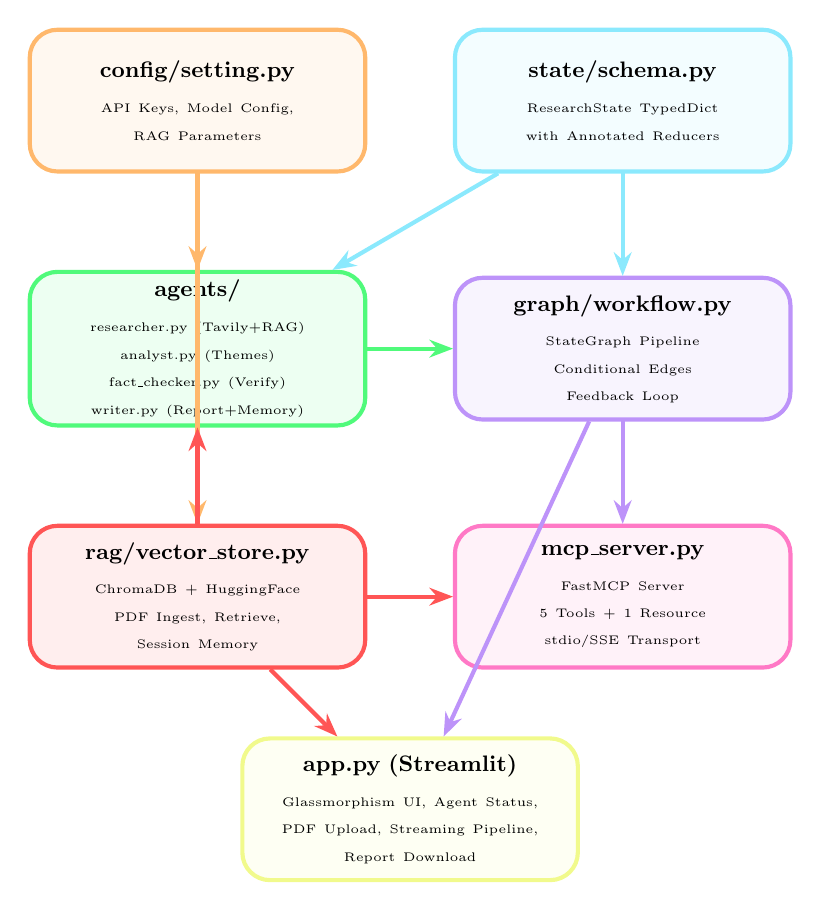
\begin{tikzpicture}[
    scale=0.9,
    transform shape,
    component/.style={draw=#1, rounded corners=10pt, fill=#1!10,
                      text width=4.5cm, align=center, minimum height=2cm,
                      font=\small, line width=1.5pt},
    conn/.style={-{Stealth[length=3mm]}, #1, line width=1.5pt},
]
    % Row 1: Config + State
    \node[component=accentorange] (config) at (0,0) {
        \textbf{config/setting.py}\\[3pt]
        {\tiny API Keys, Model Config,}\\
        {\tiny RAG Parameters}
    };
    \node[component=accentblue] (state) at (6,0) {
        \textbf{state/schema.py}\\[3pt]
        {\tiny ResearchState TypedDict}\\
        {\tiny with Annotated Reducers}
    };

    % Row 2: Agents
    \node[component=accentgreen] (agents) at (0,-3.5) {
        \textbf{agents/}\\[3pt]
        {\tiny researcher.py (Tavily+RAG)}\\
        {\tiny analyst.py (Themes)}\\
        {\tiny fact\_checker.py (Verify)}\\
        {\tiny writer.py (Report+Memory)}
    };

    % Row 2: Graph
    \node[component=accentpurple] (graph) at (6,-3.5) {
        \textbf{graph/workflow.py}\\[3pt]
        {\tiny StateGraph Pipeline}\\
        {\tiny Conditional Edges}\\
        {\tiny Feedback Loop}
    };

    % Row 3: RAG + MCP
    \node[component=accentred] (rag) at (0,-7) {
        \textbf{rag/vector\_store.py}\\[3pt]
        {\tiny ChromaDB + HuggingFace}\\
        {\tiny PDF Ingest, Retrieve,}\\
        {\tiny Session Memory}
    };
    \node[component=keyword] (mcp) at (6,-7) {
        \textbf{mcp\_server.py}\\[3pt]
        {\tiny FastMCP Server}\\
        {\tiny 5 Tools + 1 Resource}\\
        {\tiny stdio/SSE Transport}
    };

    % Row 4: UI
    \node[component=string] (ui) at (3,-10) {
        \textbf{app.py (Streamlit)}\\[3pt]
        {\tiny Glassmorphism UI, Agent Status,}\\
        {\tiny PDF Upload, Streaming Pipeline,}\\
        {\tiny Report Download}
    };

    % Connections
    \draw[conn=accentorange] (config) -- (agents);
    \draw[conn=accentorange] (config) -- (rag);
    \draw[conn=accentblue] (state) -- (agents);
    \draw[conn=accentblue] (state) -- (graph);
    \draw[conn=accentgreen] (agents) -- (graph);
    \draw[conn=accentred] (rag) -- (agents);
    \draw[conn=accentpurple] (graph) -- (ui);
    \draw[conn=accentpurple] (graph) -- (mcp);
    \draw[conn=accentred] (rag) -- (ui);
    \draw[conn=accentred] (rag) -- (mcp);
\end{tikzpicture}
\end{center}

\begin{notebox}
\textbf{Key Takeaways:}
\begin{enumerate}
\item \textbf{Modular Architecture:} Har component independent hai. Koi bhi agent replace/add kar sakte ho bina baaki code change kiye.
\item \textbf{Shared State Pattern:} TypedDict with reducers --- safe, typed, accumulating data flow.
\item \textbf{Feedback Loop:} Self-correcting pipeline with bounded revisions.
\item \textbf{RAG Integration:} Documents + Memory --- system time ke saath smarter hota hai.
\item \textbf{MCP Protocol:} Universal AI tool access --- one system, many clients.
\item \textbf{Zero Cost:} Free Groq + Tavily + Local Embeddings + ChromaDB.
\item \textbf{Production Ready:} Error handling, graceful degradation, configurable via env vars.
\end{enumerate}
\end{notebox}

\vfill
\begin{center}
\color{accentpurple}\rule{0.8\textwidth}{2pt}\\[10pt]
{\Large\bfseries\color{accentpurple} ``Jo samajh ke padhega, woh interview mein chhaa jayega!''}\\[5pt]
{\color{comment}\small Notes Generated for Multi-Agent Research Orchestrator Project}\\
{\color{comment}\small \today}
\end{center}


%=======================================================================

%=======================================================================

%=======================================================================

%=======================================================================
% CHAPTER 11: AUTH-FIRST DJANGO REST FRAMEWORK BACKEND & DOCKER DEPLOYMENT
%=======================================================================
\clearpage
\section{Chapter 11: Auth-First Django REST Framework Backend, Port 8080 \& System Architecture}

\begin{notebox}
\textbf{\faRocket\ Chapter Goal:} Is chapter mein hum Multi-Agent Research Orchestrator ke \textbf{Backend Layer} ko deep dive mein samjhenge. Pehle project sirf Client-side Streamlit + LangGraph standalone mode mein chala raha tha. Lekin production-grade enterprise system banane ke liye humne ek \textbf{Auth-First Django REST Framework (DRF) Backend} integrate kiya hai jo Port 8080 par chalta hai, Token-based Authentication, Service Layer Abstraction, User-Isolated Database Storage, aur Docker Containerization provide karta hai.
\end{notebox}

\subsection{11.1 Backend Architecture Overview: Why Django DRF?}

Humne system ko \textbf{Microservice-style Architecture} mein separate kiya hai taaki UI presentation layer, authentication, data persistence, aur AI multi-agent orchestration cleanly decoupled rahein:

\begin{center}
\resizebox{0.92\textwidth}{!}{%
\begin{tikzpicture}[
    node distance=1.4cm and 1.5cm,
    block/.style={draw=accentpurple, fill=accentpurple!10, rectangle, rounded corners=6pt, inner sep=10pt, font=\small\bfseries, align=center, text width=6cm},
    service/.style={draw=accentblue, fill=accentblue!10, rectangle, rounded corners=6pt, inner sep=10pt, font=\small\bfseries, align=center, text width=6cm},
    db/.style={draw=accentgreen, fill=accentgreen!10, cylinder, shape border rotate=90, aspect=0.25, inner sep=8pt, font=\small\bfseries, align=center, text width=5cm},
    engine/.style={draw=accentorange, fill=accentorange!10, rectangle, rounded corners=6pt, inner sep=10pt, font=\small\bfseries, align=center, text width=5cm},
    line/.style={draw=accentpurple, ->, >=stealth, line width=1.5pt}
]

% Level 1: Client
\node [block] (streamlit) {\faDesktop\ Streamlit UI Frontend Client\\{\small (Port 8501 / Glassmorphic Auth Gateway)}};

% Level 2: Backend API
\node [service, below=1.5cm of streamlit] (drf) {\faServer\ Django REST Framework API\\{\small (Port 8080 / Gunicorn Auth Server)}};

% Level 3 Left: Database
\node [db, below left=1.8cm and 0.3cm of drf] (sqlite) {\faDatabase\ SQLite / PostgreSQL\\{\small (User Auth, Tasks, Benchmarks)}};

% Level 3 Right: Service Layer & Engine
\node [engine, below right=1.8cm and 0.3cm of drf] (service) {\faCogs\ Service Abstraction Layer\\{\small (\texttt{services.py} $\rightarrow$ LangGraph Engine)}};

% Connections with clean side labels
\draw [line] (streamlit) -- node[right=5pt, font=\footnotesize\bfseries\color{accentpurple}] {1. HTTP REST / Token Auth} (drf);
\draw [line] (drf.south west) -- node[left=5pt, font=\footnotesize\bfseries\color{accentgreen}] {2a. ORM Queries} (sqlite.north);
\draw [line] (drf.south east) -- node[right=5pt, font=\footnotesize\bfseries\color{accentorange}] {2b. Execute Service} (service.north);

\end{tikzpicture}
}
\end{center}

\subsubsection{Core Backend Architectural Principles:}
\begin{enumerate}
    \item \textbf{Auth-First Security Gateway:} Unauthenticated users research pipeline ko run nahi kar sakte. Client sabse pehle \texttt{POST /api/v1/auth/login/} request bhej kar DRF Auth Token obtain karta hai, jo har request ke \texttt{Authorization: Token <key>} header mein bheja jata hai.
    \item \textbf{Port 8080 Dedicated Deconfliction:} machine par Port 8000 pehle se kisi aur DRF project (e.g. E-Commerce Platform) se occupied hone ki vajah se \texttt{404 Page Not Found} aara ha tha. Humne Orchestrator Backend ko explicitly dedicated **Port 8080** (\texttt{http://127.0.0.1:8080/api/v1/}) par configure kiya.
    \item \textbf{Service Layer Abstraction Pattern (\texttt{services.py}):} REST API Views ko directly LangGraph workflow engine se tight-couple karne ke bajaye, saari orchestration logic \texttt{ResearchOrchestratorService} class ke andar encapsulate ki gayi hai.
    \item \textbf{Strict Multi-Tenant User Isolation:} Har database query mein \texttt{filter(user=request.user)} enforce kiya jata hai. Isse User A kabhi bhi User B ke research tasks ya evaluation benchmark reports ko nahi dekh sakta.
\end{enumerate}

\clearpage
\subsection{11.2 Database Schema \& Domain Models (\texttt{backend/api/models.py})}

Backend persistence layer mein do core domain models design kiye gaye hain: \texttt{ResearchTask} (research sessions ke liye) aur \texttt{BenchmarkResult} (LLM evaluation benchmarks ke liye).

\begin{lstlisting}[style=pythonstyle, caption={backend/api/models.py --- Django Domain Models}]
from django.db import models
from django.contrib.auth.models import User

class ResearchTask(models.Model):
    STATUS_CHOICES = [
        ('PENDING', 'Pending'),
        ('RUNNING', 'Running'),
        ('COMPLETED', 'Completed'),
        ('FAILED', 'Failed'),
    ]

    user = models.ForeignKey(
        User, 
        on_delete=models.CASCADE, 
        related_name='research_tasks', 
        null=True, 
        blank=True
    )
    topic = models.CharField(max_length=500)
    status = models.CharField(max_length=50, choices=STATUS_CHOICES, default='PENDING')
    final_report = models.TextField(blank=True, null=True)
    execution_time_seconds = models.FloatField(default=0.0)
    word_count = models.IntegerField(default=0)
    created_at = models.DateTimeField(auto_now_add=True)

    class Meta:
        ordering = ['-created_at']

    def __str__(self):
        return f"{self.topic[:30]} ({self.status})"


class BenchmarkResult(models.Model):
    user = models.ForeignKey(
        User, 
        on_delete=models.CASCADE, 
        related_name='benchmark_results', 
        null=True, 
        blank=True
    )
    topic = models.CharField(max_length=500)
    single_agent_report = models.TextField()
    multi_agent_report = models.TextField()
    single_agent_latency = models.FloatField()
    multi_agent_latency = models.FloatField()
    single_agent_completeness = models.FloatField(default=0.0)
    multi_agent_completeness = models.FloatField(default=0.0)
    winner = models.CharField(max_length=50, default='MULTI_AGENT')
    created_at = models.DateTimeField(auto_now_add=True)

    class Meta:
        ordering = ['-created_at']

    def __str__(self):
        return f"Benchmark: {self.topic[:30]} - Winner: {self.winner}"
\end{lstlisting}

\subsubsection{Deep Technical Explanation:}
\begin{itemize}
    \item \textbf{\texttt{models.ForeignKey(User, on\_delete=models.CASCADE)}}: User account delete hone par uske saare linked research tasks aur benchmark results automatically database se cascade-delete ho jate hain (Referential Integrity).
    \item \textbf{\texttt{ordering = ['-created\_at']}}: Meta ordering parameter default SQL \texttt{ORDER BY created\_at DESC} add karta hai, jisse client side par hamesha latest tasks sabse upar dikhte hain.
    \item \textbf{\texttt{STATUS\_CHOICES}}: State machine pattern asynchronous workflow lifecycle (\texttt{PENDING} $\rightarrow$ \texttt{RUNNING} $\rightarrow$ \texttt{COMPLETED} / \texttt{FAILED}) ko track karta hai.
\end{itemize}

\clearpage
\subsection{11.3 Serializers Layer (\texttt{backend/api/serializers.py})}

DRF Serializers Python objects (ORM QuerySets) ko JSON representation mein convert (serialize) karte hain aur client se aane wale incoming HTTP payloads ko validate (deserialize) karte hain.

\begin{lstlisting}[style=pythonstyle, caption={backend/api/serializers.py --- DRF Data Serializers}]
from rest_framework import serializers
from django.contrib.auth.models import User
from .models import ResearchTask, BenchmarkResult

class UserSerializer(serializers.ModelSerializer):
    class Meta:
        model = User
        fields = ['id', 'username', 'email', 'first_name', 'last_name']


class RegisterSerializer(serializers.ModelSerializer):
    password = serializers.CharField(write_only=True, min_length=6)

    class Meta:
        model = User
        fields = ['username', 'email', 'password']

    def create(self, validated_data):
        user = User.objects.create_user(
            username=validated_data['username'],
            email=validated_data.get('email', ''),
            password=validated_data['password']
        )
        return user


class ResearchTaskSerializer(serializers.ModelSerializer):
    user = UserSerializer(read_only=True)

    class Meta:
        model = ResearchTask
        fields = '__all__'


class BenchmarkResultSerializer(serializers.ModelSerializer):
    user = UserSerializer(read_only=True)

    class Meta:
        model = BenchmarkResult
        fields = '__all__'
\end{lstlisting}

\subsubsection{Deep Technical Explanation:}
\begin{itemize}
    \item \textbf{\texttt{write\_only=True}}: Password string ko response output se security reasons ki vajah se omit kar deta hai.
    \item \textbf{\texttt{User.objects.create\_user()}}: Raw password ko plain-text ke bajaye Django ke default PBKDF2 with SHA256 hashing algorithm se securely hash karke DB mein store karta hai.
    \item \textbf{Nested Serialization (\texttt{user = UserSerializer(read\_only=True)})}: Task detail JSON response ke saath user details ko cleanly nest karke return karta hai.
\end{itemize}

\clearpage
\subsection{11.4 Service Layer Abstraction (\texttt{backend/api/services.py})}

Business Logic ko API Views se decouple karne ke liye Service Layer pattern use kiya gaya hai. Isse "Fat Views" Anti-Pattern avoid hota hai.

\begin{lstlisting}[style=pythonstyle, caption={backend/api/services.py --- Business Logic Layer}]
import time
from typing import Dict, Any, Optional
from django.contrib.auth.models import User
from .models import ResearchTask, BenchmarkResult
from graph.workflow import run_research_workflow
from evaluation.evaluator import BenchmarkEvaluator

class ResearchOrchestratorService:
    # Service handling orchestration task execution and history recording.

    @staticmethod
    def execute_research_task(topic: str, user: Optional[User] = None) -> Dict[str, Any]:
        task = ResearchTask.objects.create(
            topic=topic,
            user=user,
            status='RUNNING'
        )
        start_time = time.time()
        try:
            result = run_research_workflow(topic)
            elapsed = time.time() - start_time
            report = result.get('final_report', '')
            
            task.final_report = report
            task.status = 'COMPLETED'
            task.execution_time_seconds = round(elapsed, 2)
            task.word_count = len(report.split())
            task.save()
            
            return {
                'task_id': task.id,
                'status': 'COMPLETED',
                'report': report,
                'execution_time': task.execution_time_seconds,
                'word_count': task.word_count
            }
        except Exception as e:
            task.status = 'FAILED'
            task.save()
            raise e
\end{lstlisting}

\clearpage
\subsection{11.5 API Endpoints \& Token Authentication (\texttt{backend/api/views.py})}

\begin{lstlisting}[style=pythonstyle, caption={backend/api/views.py --- DRF Endpoint Handlers}]
from rest_framework import status
from rest_framework.views import APIView
from rest_framework.response import Response
from rest_framework.permissions import AllowAny, IsAuthenticated
from rest_framework.authtoken.models import Token
from django.contrib.auth import authenticate
from .models import ResearchTask
from .serializers import UserSerializer, RegisterSerializer, ResearchTaskSerializer
from .services import ResearchOrchestratorService

class RegisterView(APIView):
    permission_classes = [AllowAny]

    def post(self, request):
        serializer = RegisterSerializer(data=request.data)
        if serializer.is_valid():
            user = serializer.save()
            token, _ = Token.objects.get_or_create(user=user)
            return Response({
                'message': 'User registered successfully',
                'token': token.key,
                'user': UserSerializer(user).data
            }, status=status.HTTP_201_CREATED)
        return Response(serializer.errors, status=status.HTTP_400_BAD_REQUEST)


class LoginView(APIView):
    permission_classes = [AllowAny]

    def post(self, request):
        username = request.data.get('username')
        password = request.data.get('password')
        user = authenticate(username=username, password=password)
        if user:
            token, _ = Token.objects.get_or_create(user=user)
            return Response({
                'token': token.key,
                'user': UserSerializer(user).data
            })
        return Response({'error': 'Invalid credentials'}, status=status.HTTP_401_UNAUTHORIZED)


class StartResearchView(APIView):
    permission_classes = [IsAuthenticated]

    def post(self, request):
        topic = request.data.get('topic')
        if not topic:
            return Response({'error': 'Topic is required'}, status=status.HTTP_400_BAD_REQUEST)
        
        data = ResearchOrchestratorService.execute_research_task(topic=topic, user=request.user)
        return Response(data, status=status.HTTP_200_OK)


class ResearchHistoryView(APIView):
    permission_classes = [IsAuthenticated]

    def get(self, request):
        tasks = ResearchTask.objects.filter(user=request.user)
        serializer = ResearchTaskSerializer(tasks, many=True)
        return Response(serializer.data, status=status.HTTP_200_OK)
\end{lstlisting}

\clearpage
\subsection{11.6 Docker Containerization \& Deployment}

Production deployment ke liye Multi-container Docker compose orchestration set up ki gayi hai.

\begin{lstlisting}[style=bashstyle, caption={docker-compose.yml --- Production Orchestration}]
version: '3.8'

services:
  django_backend:
    build:
      context: .
      dockerfile: Dockerfile.backend
    ports:
      - "8080:8080"
    environment:
      - PORT=8080
      - GROQ_API_KEY=${GROQ_API_KEY}
      - TAVILY_API_KEY=${TAVILY_API_KEY}
    volumes:
      - ./backend/db.sqlite3:/app/backend/db.sqlite3
      - ./chroma_db:/app/chroma_db
    restart: always

  streamlit_frontend:
    build:
      context: .
      dockerfile: Dockerfile.frontend
    ports:
      - "8501:8501"
    environment:
      - BACKEND_API_URL=http://django_backend:8080/api/v1
    depends_on:
      - django_backend
    restart: always
\end{lstlisting}

\clearpage
\subsection{11.7 Backend \& Django DRF Interview Questions (Q51 -- Q65)}

\begin{notebox}
\textbf{Question 51: Tumne Streamlit Direct execution ke bajaye Django DRF backend kyun introduce kiya?}\\
\textbf{Answer:} Single-tier Streamlit apps me user authentication, persistent task history, user isolation, aur API third-party integration impossible ho jata hai. Django DRF se humein Token Authentication, ORM-managed Database persistence, Service Layer separation, aur Port 8080 REST endpoints mile jinhein external clients (web, mobile, CLI) consume kar sakte hain.
\end{notebox}

\begin{notebox}
\textbf{Question 52: Service Layer Pattern (\texttt{services.py}) ka kya benefit hai?}\\
\textbf{Answer:} Agar hum LangGraph execution logic \texttt{views.py} me likhte to views heavy aur un-testable ho jate (Fat Views antipattern). Service Layer Abstraction business logic ko HTTP request handling se decouple karta hai, jisse same logic CLI, Celery tasks, ya DRF views me reuse ki ja sakti hai.
\end{notebox}

\begin{notebox}
\textbf{Question 53: Port 8080 Collision Resolution kaise handle hua?}\\
\textbf{Answer:} Default Port 8000 par machine me pehle se E-Commerce DRF server running tha. Direct call karne par 404 Page Not Found aata tha. Humne Orchestrator Backend ko explicitly Port 8080 par configure kiya aur Streamlit frontend me API base URL update kiya.
\end{notebox}

\begin{notebox}
\textbf{Question 54: DRF me \texttt{TokenAuthentication} kaise kaam karti hai?}\\
\textbf{Answer:} Client \texttt{POST /auth/login/} par credentials bhejta hai. Server DB me User ka unique 40-character hex key Token return karta hai. Next requests me client \texttt{Authorization: Token <key>} header bhejta hai, jise DRF ka \texttt{IsAuthenticated} permission class validate karke \texttt{request.user} set karta hai.
\end{notebox}

\begin{notebox}
\textbf{Question 55: Multi-tenant Data Security / User Isolation kaise achieve kiya?}\\
\textbf{Answer:} Models me \texttt{user = models.ForeignKey(User, on\_delete=models.CASCADE)} enforce kiya aur har History endpoint me QuerySet ko strictly \texttt{ResearchTask.objects.filter(user=request.user)} se evaluate kiya, taaki user A kabhi user B ka data na dekh sake.
\end{notebox}


\end{document}